\section{Flow correlations}
\label{sec:ps:flow}
%5. Flow Correlations & Flow & PID Flow (PS)
%- Geometric fluctuations and origin of v_n vs ecc_n (Glauber, v3)
%- non-PID flow (ALICE first results)
%- PID flow (ALICE v2 scaling)
%- 2PC (CMS v_n?)
%- Event plane (ATLAS EP)
%- Explaining the ridge (2PC from 3 experiments)
%- Flow fluctuations
%- Event plane correlations
%- Success of viscous hydro
%- Comparison with RHIC
%- Flow in p+Pb (ridge, double ridge, PID)
%- Open questions

%\subsection{Introduction}

While the previous section covered physical mechanisms which induce
correlations between multiple hadrons, this section covers the
phenomenon of ``collective flow'', which leads to the correlations of
essentially all the particles in every event.
This results from the translation of anisotropies in the initial shape of the
colliding nuclei into anisotropies in momentum space, something that
would not occur if individual nucleon-nucleon collisions emitted independently
of each other.
The characterization of a ``shape'' in a final state particle distribution
is typically performed using a Fourier decomposition of the azimuthal
angle distribution of final state particles.
Of course, averaging over an ensemble of independent events would lead to
the observation of no net anisotropy.  Thus, the presence of harmonic
oscillations in the final state requires the estimation of an ``event plane''
from the particle themselves, with an axis that points in the direction of
the largest momentum flow.

While this phenomenon was observed decades ago in the collisions of large
nuclei at low energies, this was straightforward to understand as the
reinteraction of the initial baryons and the produced hadrons, which
would thermalize and evolve as a ``hadron gas''.
However, its persistence at higher energies, particularly at RHIC where the
value of $v_2$ averaged over \pT\ was approximately twice as large as it was at the
CERN SPS~\cite{Ackermann:2000tr}, surprised many who expected the hot system to become more
dilute and more weakly-interacting at higher energies.

Collective flow was a major piece of the RHIC program, and its characterization
in terms of hydrodynamics was a crucial piece of evidence in the RHIC discovery
of the strongly-coupled quark gluon plasma (sQGP)~\cite{Back:2004je,Adcox:2004mh,Adams:2005dq,Arsene:2004fa}.  
Crucial aspects of collective
flow, on the experimental and theoretical sides at RHIC, have been:
\begin{itemize}
\item Based on theoretical calculations, the average elliptic flow, scaled by the eccentricity,
is thought to reach a limiting value in the limit where
the viscosity can be ignored.  RHIC data achieved this limit both integrally (integrated over \pT)
and for $v_2(\pT)$, which rises linearly until viscous corrections become large.
\item When studied as a function of particle type, it is found that heavier particles show
a smaller $v_2$ at the same \pT\ at low \pT, while this hierarchy flips above 1.5~GeV, where protons
typically have a 50\% higher value of $v_2$.  This behavior has been explained by the hadronization of
the system via constituent quarks which recombine into baryons with $v_2$(baryon)=$(3/2) \times v_2$(meson)~\cite{Adare:2006ti,Fries:2003vb}.
\item The deviations from ideal behavior can be systematically calculated by viscous corrections, and
all RHIC data point to a small but significant value of the ratio of shear viscosity to entropy density ($\eta/s$)~\cite{Luzum:2008cw}.
\item While difficult to calculate in the strongly-coupled limit, where the approximations required for kinetic theory break down, AdS/CFT-based calculations have shown that a wide range of strongly-coupled systems have a lower-bound on
$\eta/s = 1/4\pi$~\cite{Kovtun:2004de}.  The RHIC experimental data suggest values of 1-2 times this bound, although estimates are limited
by theoretical uncertainties related to the modeling of the initial state~\cite{Luzum:2008cw}.
\item When studying smaller systems (particularly Cu+Cu), it was found that accounting for the event-by-event position of the nucleons in the nuclear wave functions showed scaling in the quantity $v_2/\epsilon$ between Cu+Cu and Au+Au, when
plotted as a function of the transverse density of charged particles at mid-rapidity, estimated by $dN_{ch}/d\eta/S$,
where $S$ is the overlap area of the two nuclei~\cite{Alver:2008zza}.
\end{itemize}

\subsection{Methods}
\label{subsect:pas:flow:methods}
Harmonic flow is a global modulation of essentially all of the particles in an event relative to an event plane
appropriate to each harmonic.  However, there are additional sources of multi-particle correlations, some which
lead to global correlations (momentum conservation) and others which only lead to correlations local in angular space
(e.g. resonance decays and jets).  Thus, care must be taken to minimize such ``non flow'' correlations.

One of the earliest methods for measuring flow was the ``event plane'' method, which calculates an event plane using
a forward detector and correlates all particles with this event plane, based on the so-called ``Q-vector'' for each order $n$~\cite{Poskanzer:1998yz}:
\begin{equation}
\end{equation}
From this, the $n$-th order event plane $\Psi_n$ is simply determined as the angle of the Q-vector itself.
From the definition of the Q-vector, the angle is $n$-fold ambiguous, but this has no effect on the extracted
$v_n$ coefficient, which is defined as
\begin{equation}
v_n = \frac{v^{obs}_n}{\mathrm{Res}\{ n \Psi_n \}} = \frac{ \langle \cos ( n [\varphi - \Psi_n] ) \rangle }{ \langle \cos ( n [\varphi_n - \Psi_n] ) \rangle    }
\end{equation}
where $\varphi_n$ is the direction of the true event plane.  The latter quantity cannot be observed directly and so the
resolution parameter must be derived from comparison of different detector regions.  This is typically done by comparing
symmetric pseudorapidity regions separated from the region being measured:
\begin{equation}
\mathrm{Res} \{ n \Psi_n^{\mathrm{P(N)}} \} =
\langle \cos n ( \Psi_n^{\mathrm{P(N)}} - \Psi_n ) \rangle =
\sqrt{ \langle \cos n ( \Psi_n^{\mathrm{P}} - \Psi_n^{\mathrm{N}} ) \rangle }
\end{equation}
Non-flow contamination is typically most difficult to control when the subevents used to determine the event plane
and resolution are close in $\eta$ to each other or close to the measured particles.
%
Another method is to use multi-particle cumulants to explicitly remove lower order 
correlations~\cite{Borghini:2000sa,Borghini:2001vi,Borghini:2001zr,Bilandzic:2010jr}.
These can be calculated either from a generating function formalism, or through moments of the Q-vector itself.
They are more or less sensitive to non-flow depending on the order of the cumulant.  For example, the two-particle
cumulant is quite sensitive to effects from resonance decay and jet fragmentation.  However, the four particle
cumulants are generally much less so, since it explicitly removes short-range two particle correlations.
%
A third method is to use the ``Lee-Yang zeroes'' approach, which accounts for correlations of all lower orders using a
different generating function~\cite{Bhalerao:2003yq,Borghini:2004ke}.  
The method relates the zeros of a complex function to the magnitude of the relevant
flow harmonics.  While the method is thought to be robust against most sources of non-flow, it is particularly sensitive to
multiplicity fluctuations, and so is calculated using event samples with similar multiplicities within a given
centrality interval.  Theses subsamples are then averaged within the desired centrality interval to give the final result.

Another complementary approach to measuring flow coefficients is to
measure two-particle correlations as a function of $\Delta\eta$ and
$\Delta\varphi$, and decompose them into harmonics using either fits
or discrete Fourier
transforms~\cite{ATLAS:2012at,Aamodt:2011by,ALICE:2011ab}.  If
the two-particle distribution can be factorized into the product of
single particle distributions, $1+\sum_n v_n \cos(n[\varphi-\Psi_n])$,
then the two particle distribution, for $\Delta\eta$ regions selected
to suppress jets and other sources of non-flow, takes the form:
\begin{equation}
\frac{dN_{\mathrm{pair}}}{d\Delta\varphi} \propto 1 + 2 \sum_n^{\infty} v_{n,n}(p_T^a,p_T^b) \cos n\Delta\varphi
\end{equation}
Where $v_{n,n}(p_T^a,p_T^b) = v_n(p_T^a) v_n(p_T^b)$.  Results using
two-particle correlations and direct measurements of flow coefficients
typically give similar results if this factorized form holds true for
experimental data.

\subsection{Elliptic flow}
\begin{figure}[!tb]
\begin{center}
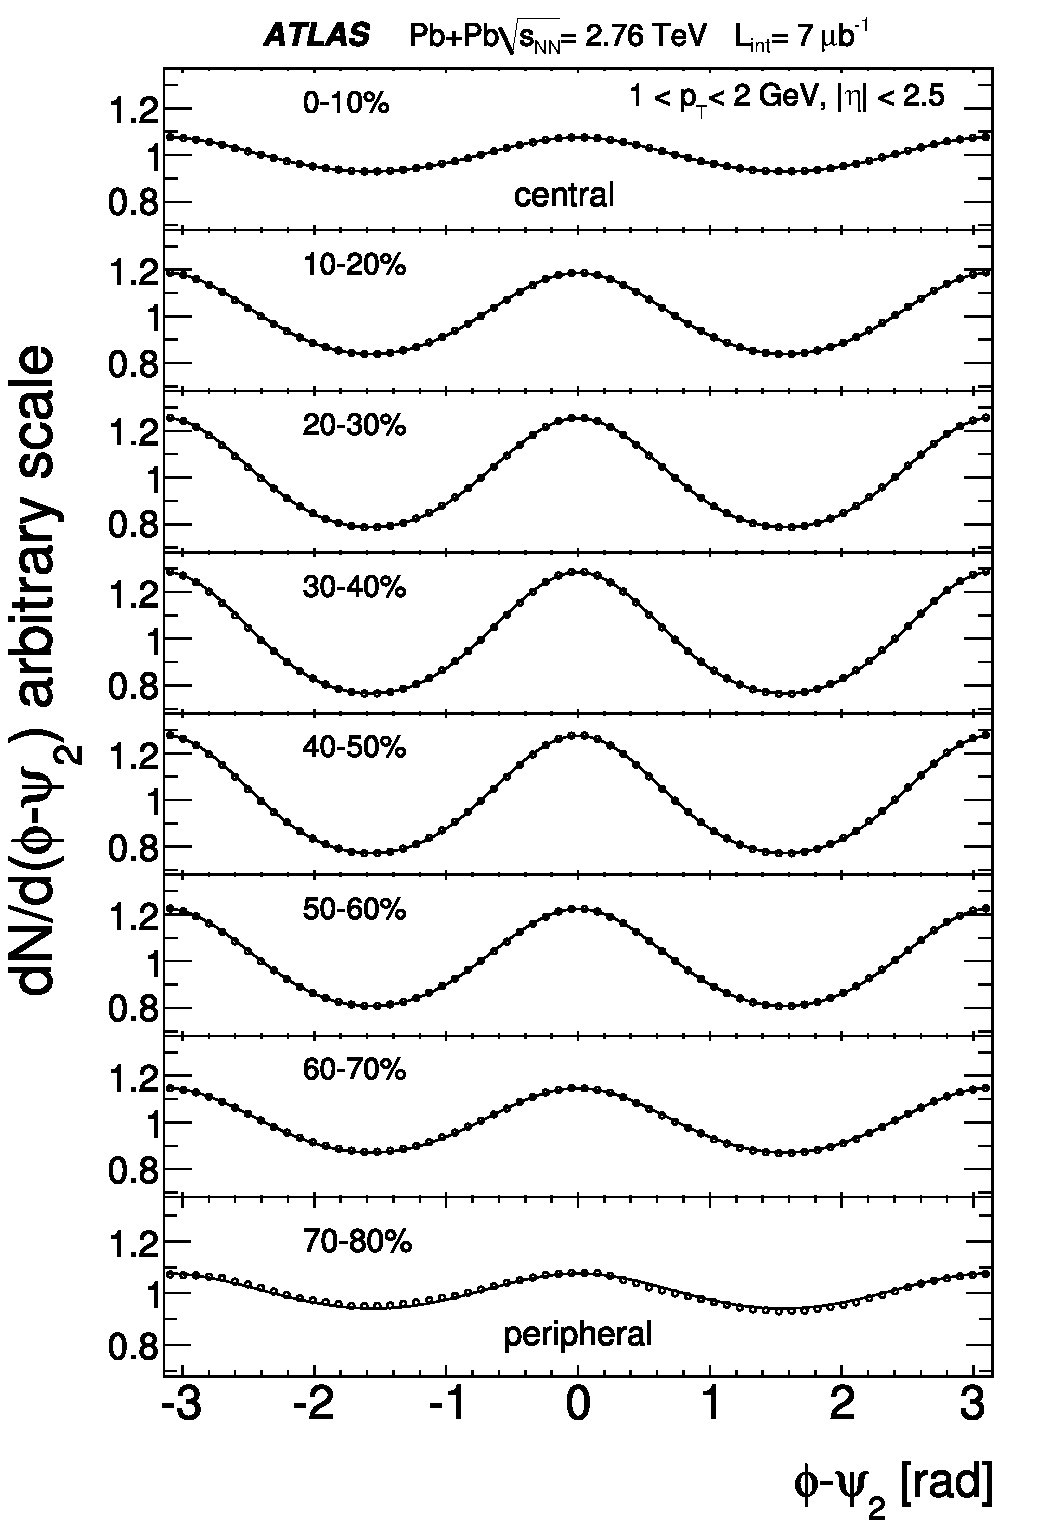
\includegraphics[height=0.49\textwidth]{flowcorrelations_figs/atlas_v2_fig_02.pdf}
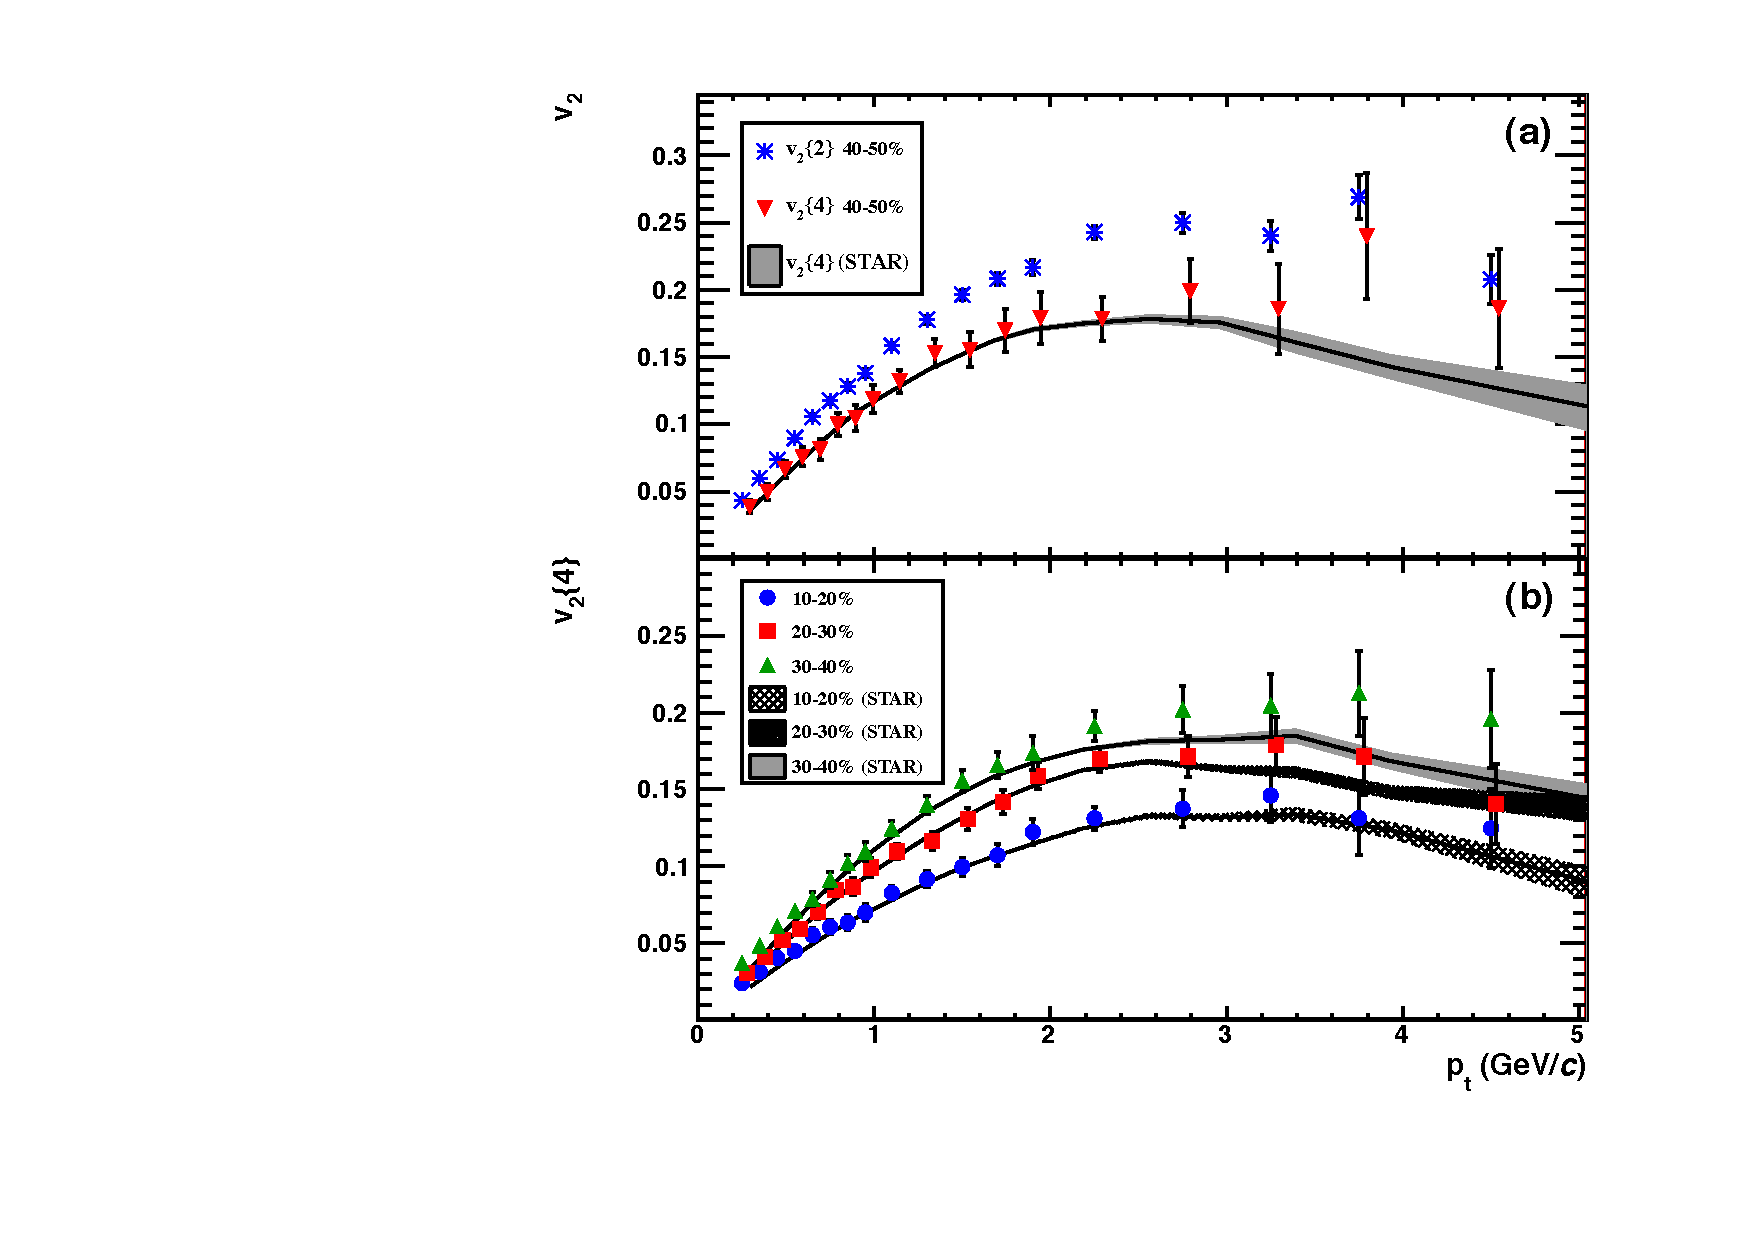
\includegraphics[height=0.49\textwidth]{flowcorrelations_figs/fig2.pdf}
\caption[]{(left) ATLAS data showing the evolution of anisotropy relative to the reaction plane, as a function of centrality~\cite{ATLAS:2011ah} (right) First ALICE data on \vtwo\ in \PbPb\ collisions at the LHC~\cite{Aamodt:2010pa}.}
\label{fig:pas:fc:firstresults}
\end{center}
\end{figure}
The first LHC data on elliptic flow was released by the ALICE collaboration soon after the first collisions,
and is shown in Figure~\ref{fig:pas:fc:firstresults}.
The elliptic flow was estimated using three methods: 2-particle cumulants ($v_2\{2\}$), 4-particle cumulants ($v_2\{4\}$)
and Lee-Yang Zeros (LYZ).  The first method is known to be sensitive to correlation from jets, which have
a larger contribution at the LHC than at RHIC, and the latter method was only used for integral flow.
The integral flow was found to be larger than that measured at RHIC, but only by about 15-20\%.
What was surprising was that, as a function of \pT\ (but only measured out to 4~GeV)
the magnitude of $v_2$ was found to be quantitatively very similar to that measured in
the STAR experiment at RHIC, using similar cumulant methods.
Although a similar scaling has been observed in the very low energy
data on inclusive $v_2(\pT)$ from STAR taken during the recent RHIC energy scan,
there is no fundamental understanding yet of how this scaling arises.
It suggests that most of the variation in the integral elliptic flow results from the change in the spectral shape
of inclusive hadrons.
A hydrodynamic calculation by Luzum was able to reproduce this result soon after its release,
based on a scaling of the initial energy density according to the measured charged-particle
multiplicity, and assuming no change in the medium transport properties~\cite{Luzum:2010ag}.
The first $v_2$ measurement at higher \pT\ was performed by ATLAS~\cite{ATLAS:2011ah},
showing the transition from the low \pT\ behavior,
understood by viscous hydrodynamics, to the higher \pT\ values presumably explained by the path-length dependence of
energy loss of jets.
By comparison with PHENIX data on $\pi^0$ particles~\cite{Adare:2010sp}, this shows that the scaling of $\vtwo(\pT)$ with beam energy 
extends to high \pT\ as well,
albeit within the large statistical errors of the lower-energy measurement.

\begin{figure}[!tb]
\begin{center}
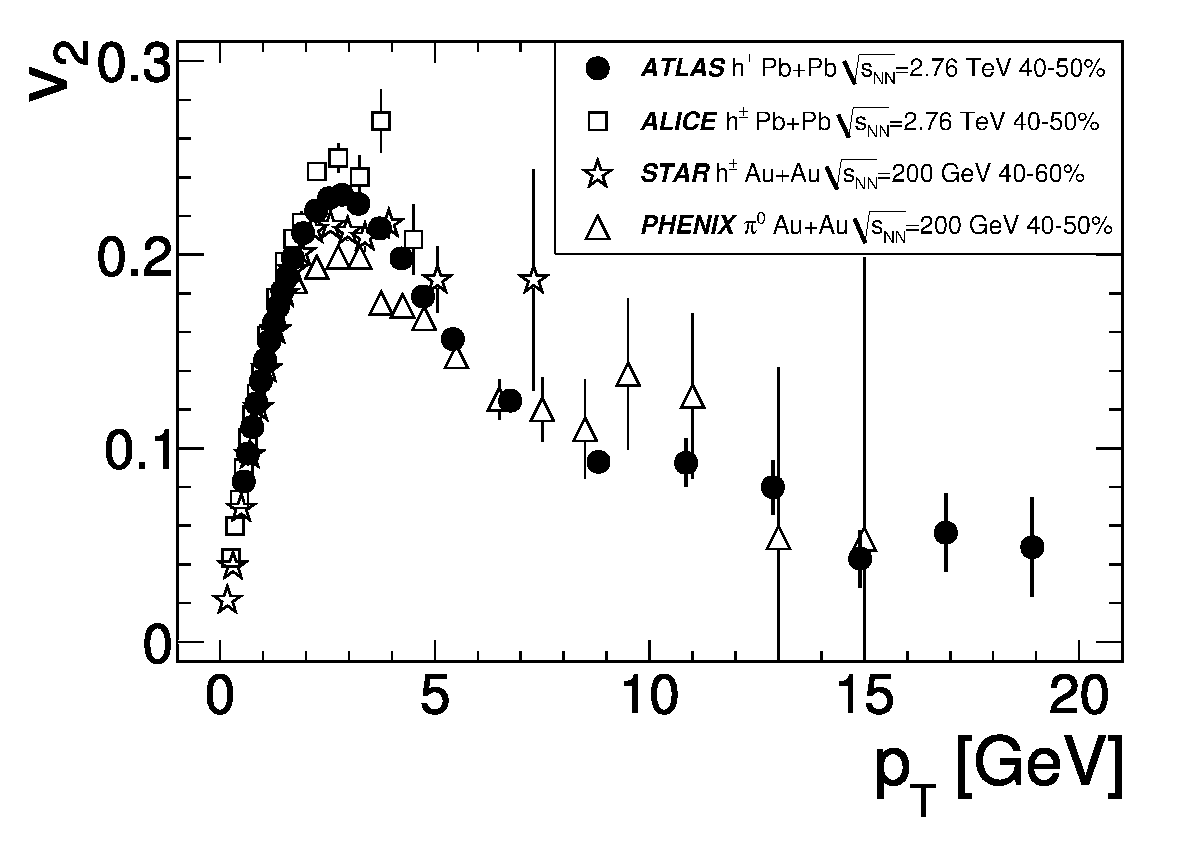
\includegraphics[width=0.55\textwidth]{flowcorrelations_figs/atlas_v2_fig_06.pdf}
\raisebox{.5cm}{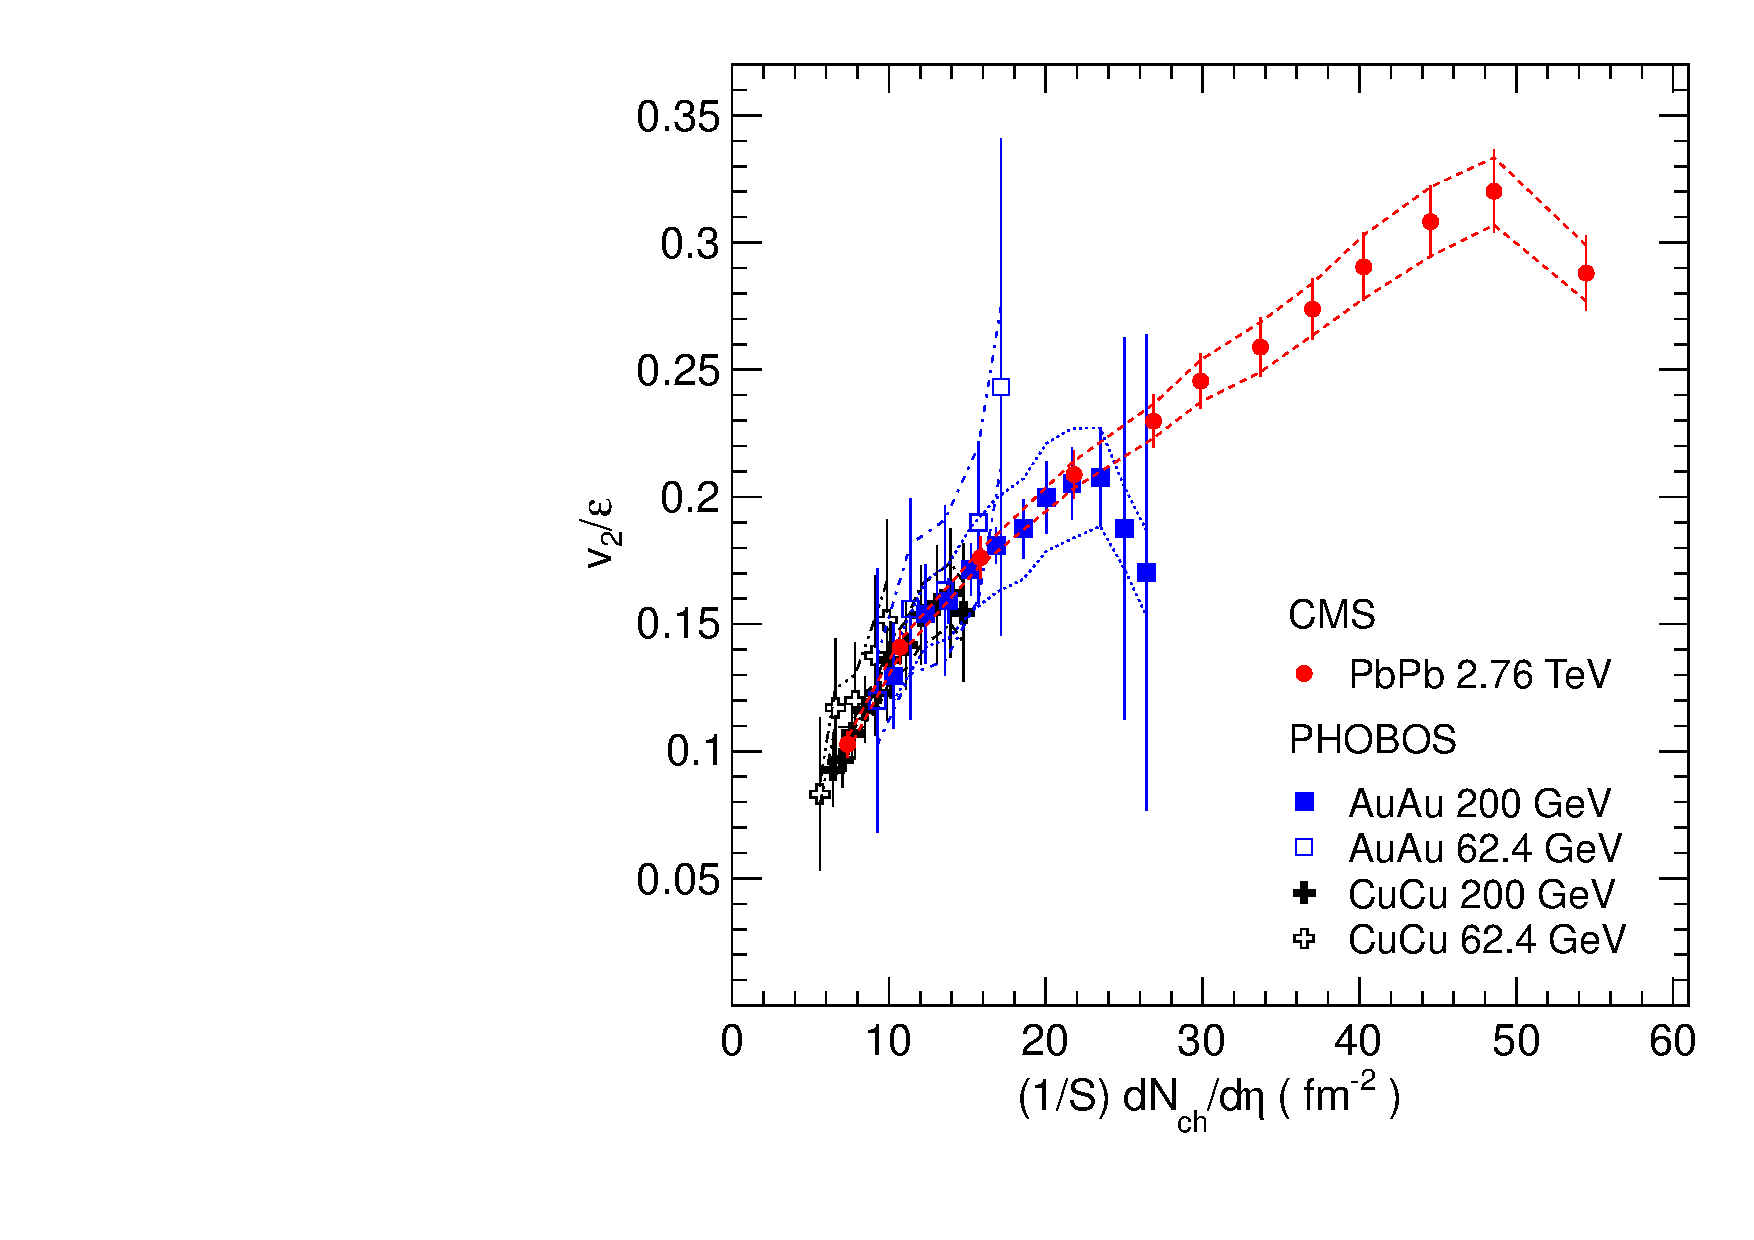
\includegraphics[width=0.39\textwidth]{flowcorrelations_figs/v2eps_dNdetaoverS_PHOBOS.pdf}}
\caption[]{(left) ATLAS data showing the invariance of $\vtwo( \pT )$
  with beam energy~\cite{ATLAS:2011ah} (right) CMS compilation showing
  the observed scaling of $\vtwo /\epsilon$ vs. $(1/S)
  dN_{ch}/d\eta$~\cite{Chatrchyan:2012ta}.}
\label{fig:pas:fc:scaling}
\end{center}
\end{figure}
The dependence of the inclusive elliptic flow on the initial state geometry was studied carefully by CMS, who
performed a careful extrapolation of the integral $v_2$ down to $\pT>0$~GeV, using simultaneous measurements of
$dN/d\pT$, to match with the lower energy PHOBOS data.
To factor out the initial shape and size of the overlap region, a Monte Carlo Glauber model was used to match
the centrality selections made with the CMS forward calorimeter.
From these, the eccentricity and overlap area were calculated according to the definitions from
subsection~\ref{subsect:pas:flow:methods}.  The CMS data, shown superimposed on data from RHIC, is shown in
Figure~\ref{fig:pas:fc:scaling}(right), and overlaps the PHOBOS Au+Au and 
Cu+Cu data in the most peripheral collisions and
shows a continuous rise in the more central collisions, except perhaps in the most central interval.

\begin{figure}[!tb]
\begin{center}
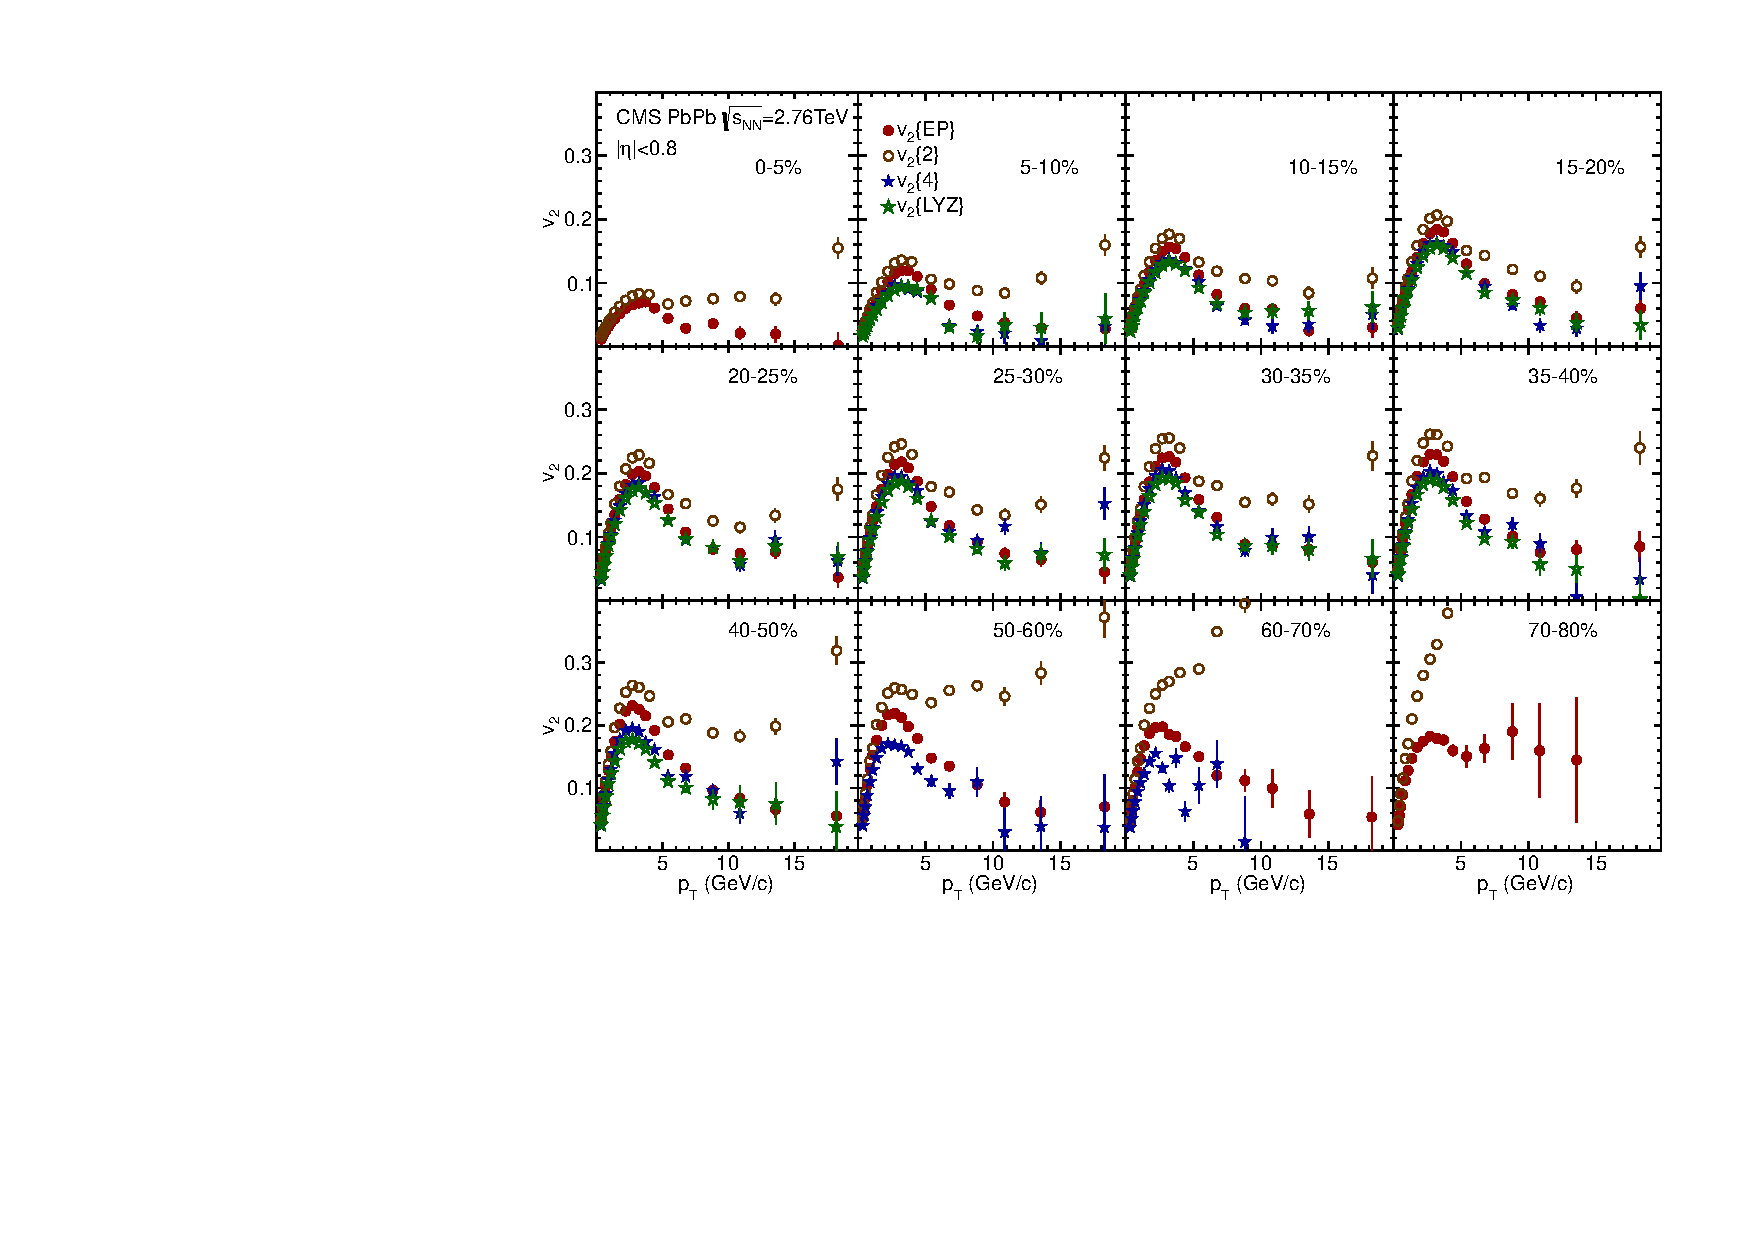
\includegraphics[width=0.8\textwidth]{flowcorrelations_figs/v2_pt_12cen_4methods.pdf}
\caption[]{
CMS data showing $\vtwo(\pT)$ in centrality intervals, using four different methods of extracting
$\vtwo$: event plane (EP), 2-particle cumulants, 4-particle cumulants, and Lee-Yang Zeros~\cite{Chatrchyan:2012ta}.
}
\label{fig:pas:fc:methods}
\end{center}
\end{figure}

The CMS data shown in Figure~\ref{fig:pas:fc:methods} illustrates the $\pT$ and centrality dependence of
$v_2(\pT)$, comparing directly the different methods of flow reconstruction used for $v_2$.
While it is clear that the 2-particle cumulant is the most contaminated by non-flow, particularly at high $\pT$,
one also observes some systematic differences between all of the methods, particularly where the flow
is the strongest.

\begin{figure}[!tb]
\begin{center}
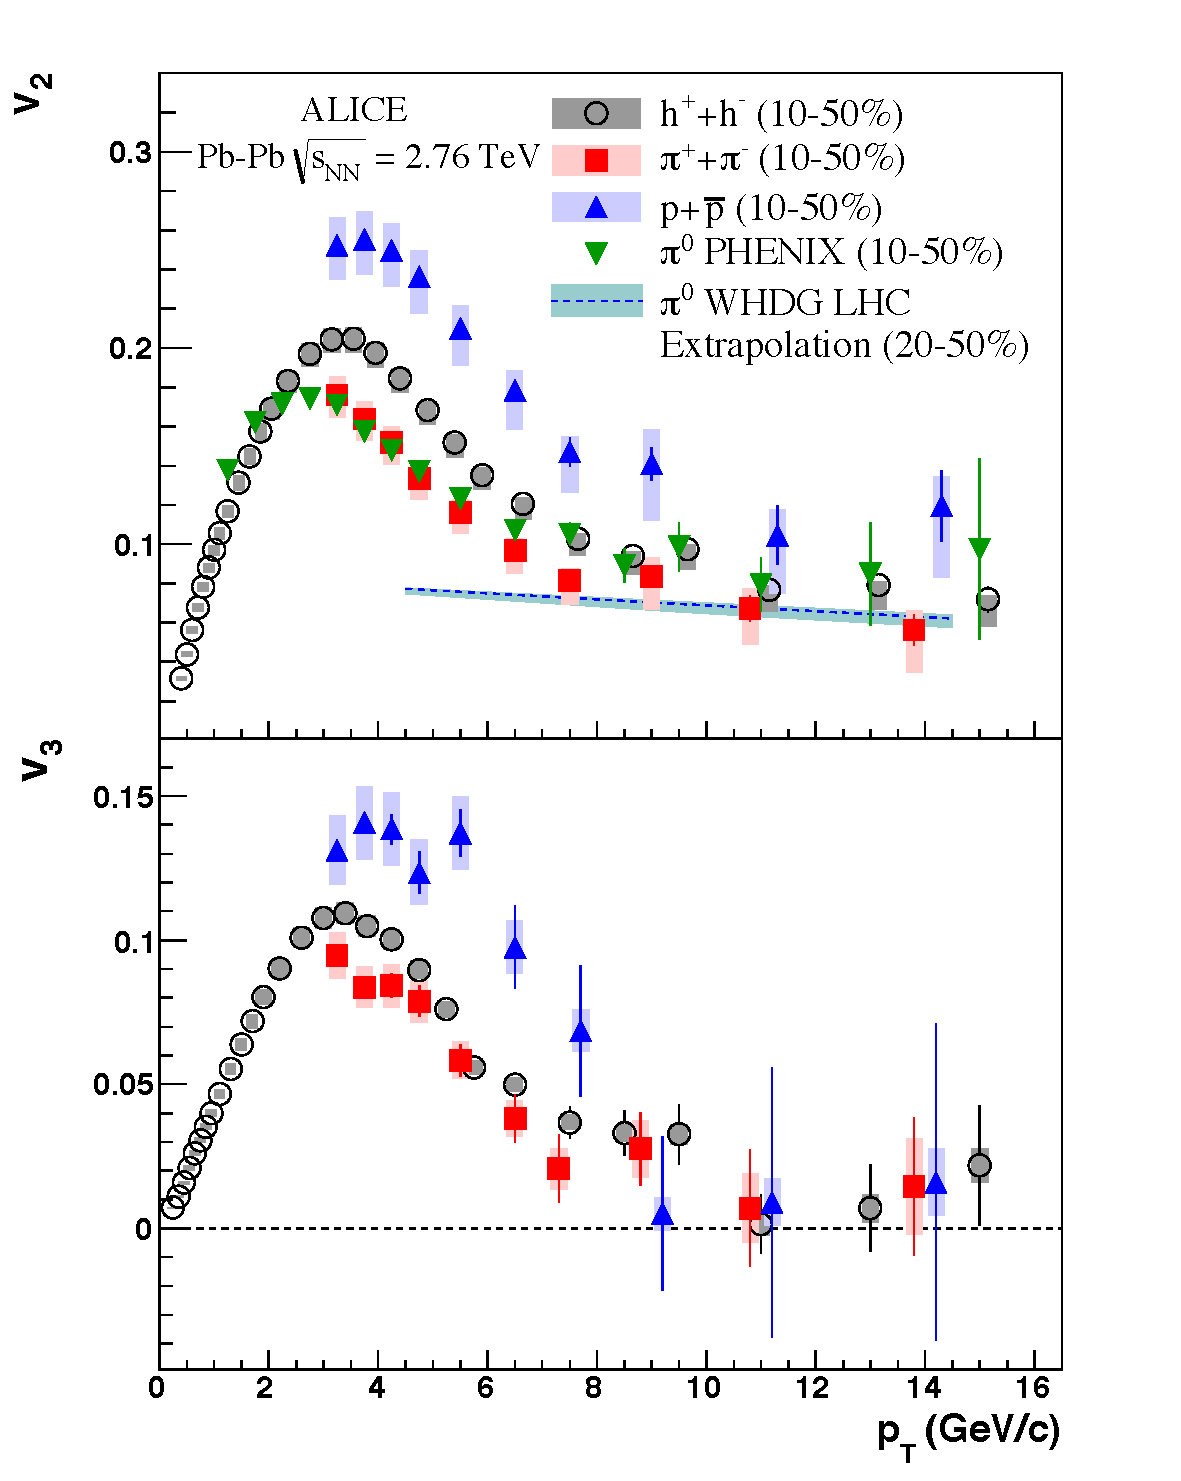
\includegraphics[width=0.35\textwidth]{flowcorrelations_figs/alice_fig5_vn_pid.pdf}
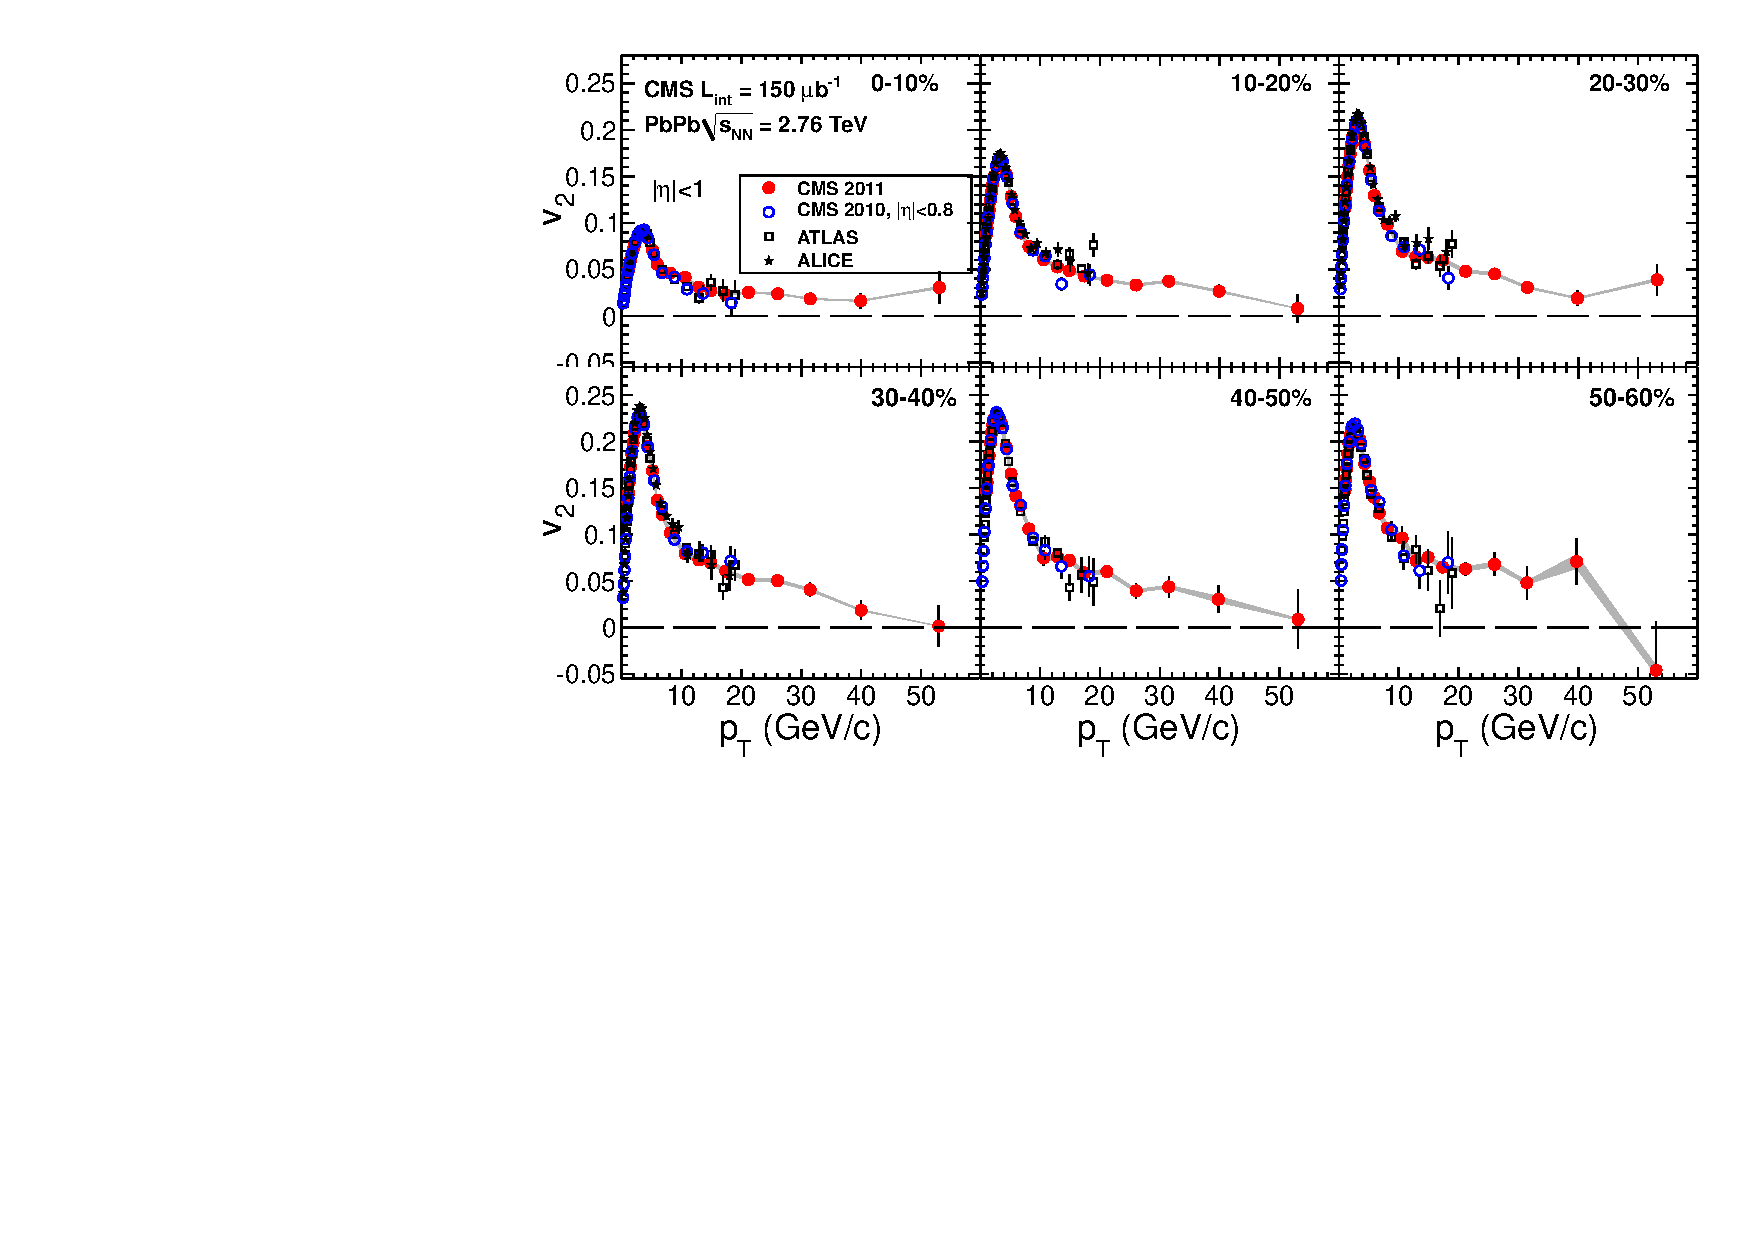
\includegraphics[width=0.63\textwidth]{flowcorrelations_figs/v2_pt_ep_atlas_alice_eta0-1_band_v5.pdf}
\caption[]{(left) ALICE data showing $\vtwo(\pT)$ for identified
  hadrons, for $|\eta|<0.8$~\cite{Abelev:2012di} (right) CMS data
  showing the $\vtwo$ for unidentified hadrons at very high \pT, out
  to 50~GeV~\cite{Chatrchyan:2012xq}}
\label{fig:pas:fc:highpt}
\end{center}
\end{figure}
The previous results have all been for unidentified hadrons.  This choice provides the largest phase
space coverage (particularly in $\pT$) and allows for comparisons between experiments with different particle
identification capabilities.  However, a study separating the different hadron species is crucial,
given the previous measurements at RHIC showing the strong differences between them.
The ALICE data showing identified particles (separated using the $dE/dx$ measured in the ALICE TPC) for $\pT>3$~GeV
is shown in Figure~\ref{fig:pas:fc:highpt}(left).  The charged pion data on $v_2(\pT)$ is quantitatively similar to
the PHENIX $\pi^0$ data over the $\pT$ range where they overlap.  The proton-antiproton $v_2$ are found to be
substantially larger than the pion values over the measured $\pT$ range, although it is clear that the peak-plateau
structure seen in the inclusive hadron data is not a feature shown only 
by one particular hadron type.
Also, at the highest $\pT$ measured, the protons and pions are quite close, although the protons remain
systematically higher out to 14~GeV.
CMS extends the hadron $\pT$ range out to the full range provided by the LHC in 2011, using a high $\pT$
high level track trigger.  The data, shown in Figure~\ref{fig:pas:fc:highpt}(right), show that the
plateau observed setting in above 6~GeV extends out to at least 50~GeV, with only mild decreases observed within
the stated uncertainties.

\begin{figure}[!tb]
\begin{center}
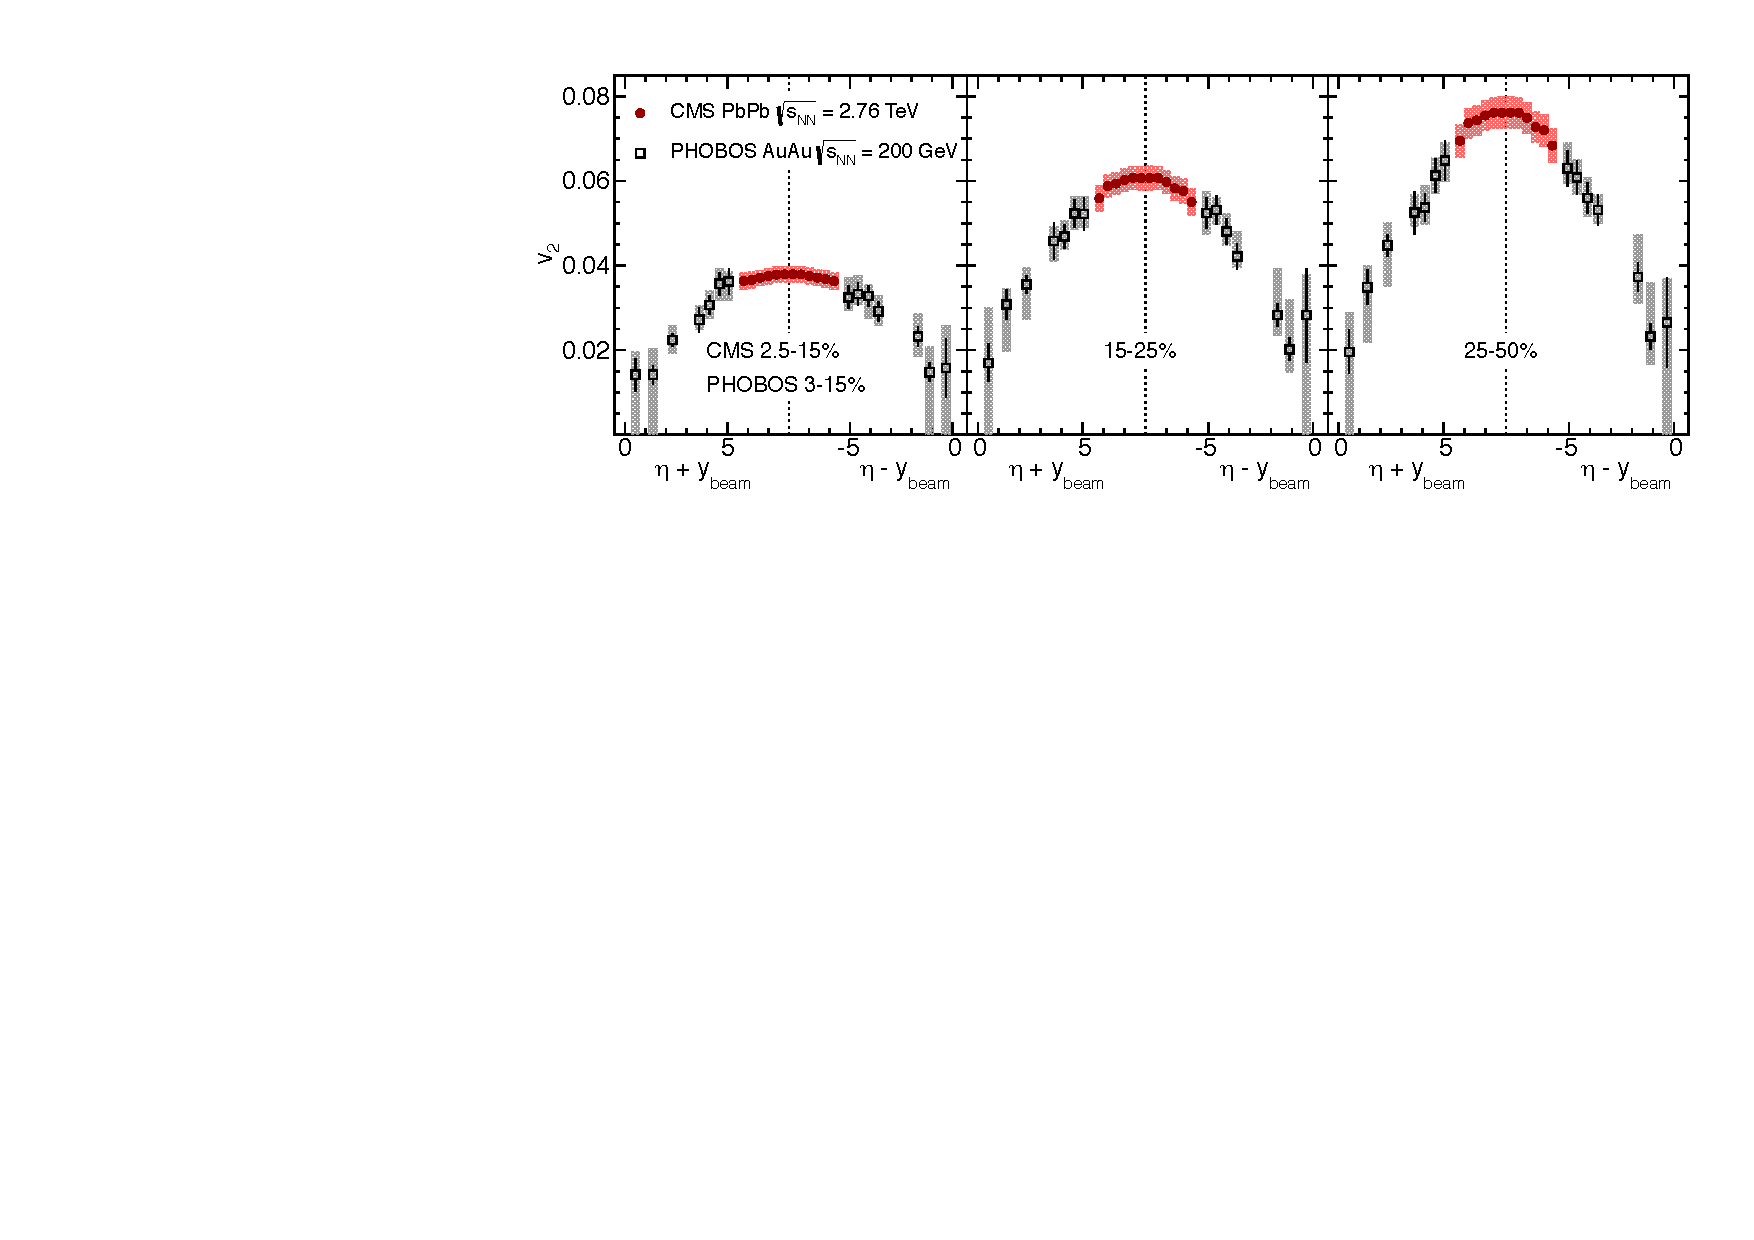
\includegraphics[width=0.98\textwidth]{flowcorrelations_figs/v2_etashifted_3cen_PHOBOS.pdf}
\caption[]{
CMS data showing $\vtwo$ for unidentified hadrons as a function of $\eta - y_{\mathrm{beam}}$, averaged over $0 <\pT < 3$~GeV (using an extrapolation procedure to cover $\pT <300$ Mev).
Results are compared to data from $\sqrt{s_{NN}}=200$~GeV
at large $\eta$ from the PHOBOS experiment at RHIC~\cite{Chatrchyan:2012ta}.
}
\label{fig:pas:fc:limfrag}
\end{center}
\end{figure}
Another intriguing way to compare with the lower energy data is suggested by studies performed by the PHOBOS
collaboration, which found that the integrated $v_2(\eta)$ is the same for different colliding beam energies,
when plotted in the rest frame of one of the projectiles.  This is the phenomenon of so-called
``limiting fragmentation'', where many quantities are found to depend only on their rapidity relative to either
beam or projectile.
Figure~\ref{fig:pas:fc:limfrag} shows $v_2(\eta)$ as a function of $\eta - y_{\mathrm{beam}}$ (in the forward
hemisphere) and $\eta + y_{\mathrm{beam}}$ in the backward hemisphere.
While the CMS and PHOBOS data points do not overlap in any measured region, they appear to be continuous
in the forward LHC kinematics and the mid-rapidity RHIC kinematics.
However, it is clear that the behavior of the CMS data is much more suggestive of a boost-invariant central
plateau, while the PHOBOS data did not show similar behavior.

\subsection{Higher order harmonics}

\begin{figure}[!tb]
\begin{center}
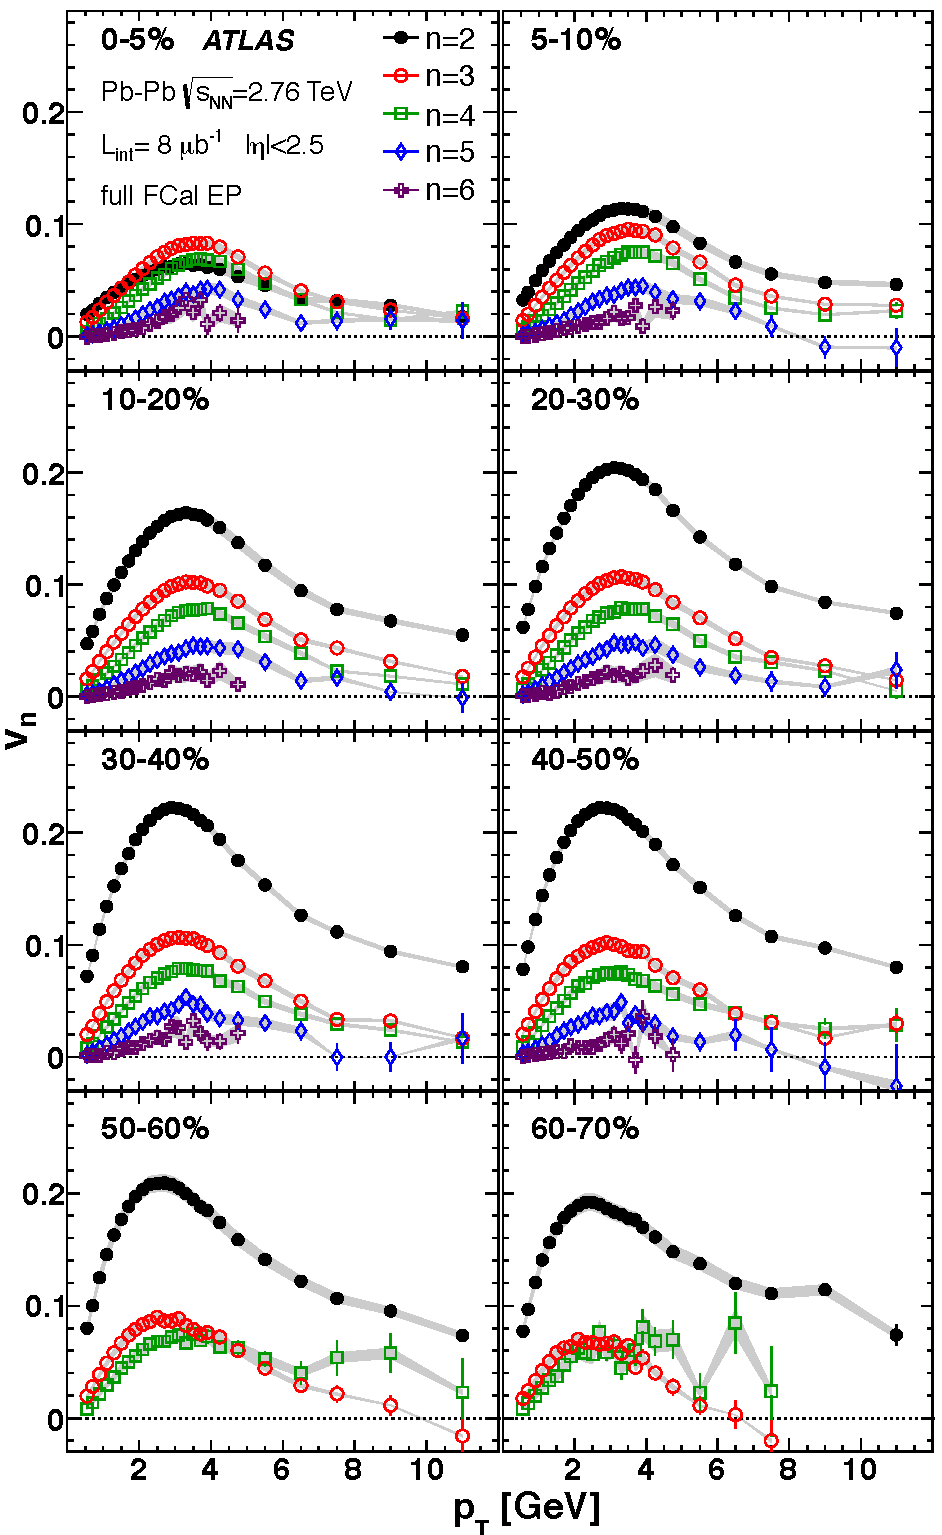
\includegraphics[height=0.6\textwidth]{flowcorrelations_figs/atlas_vn_fig_04.pdf}
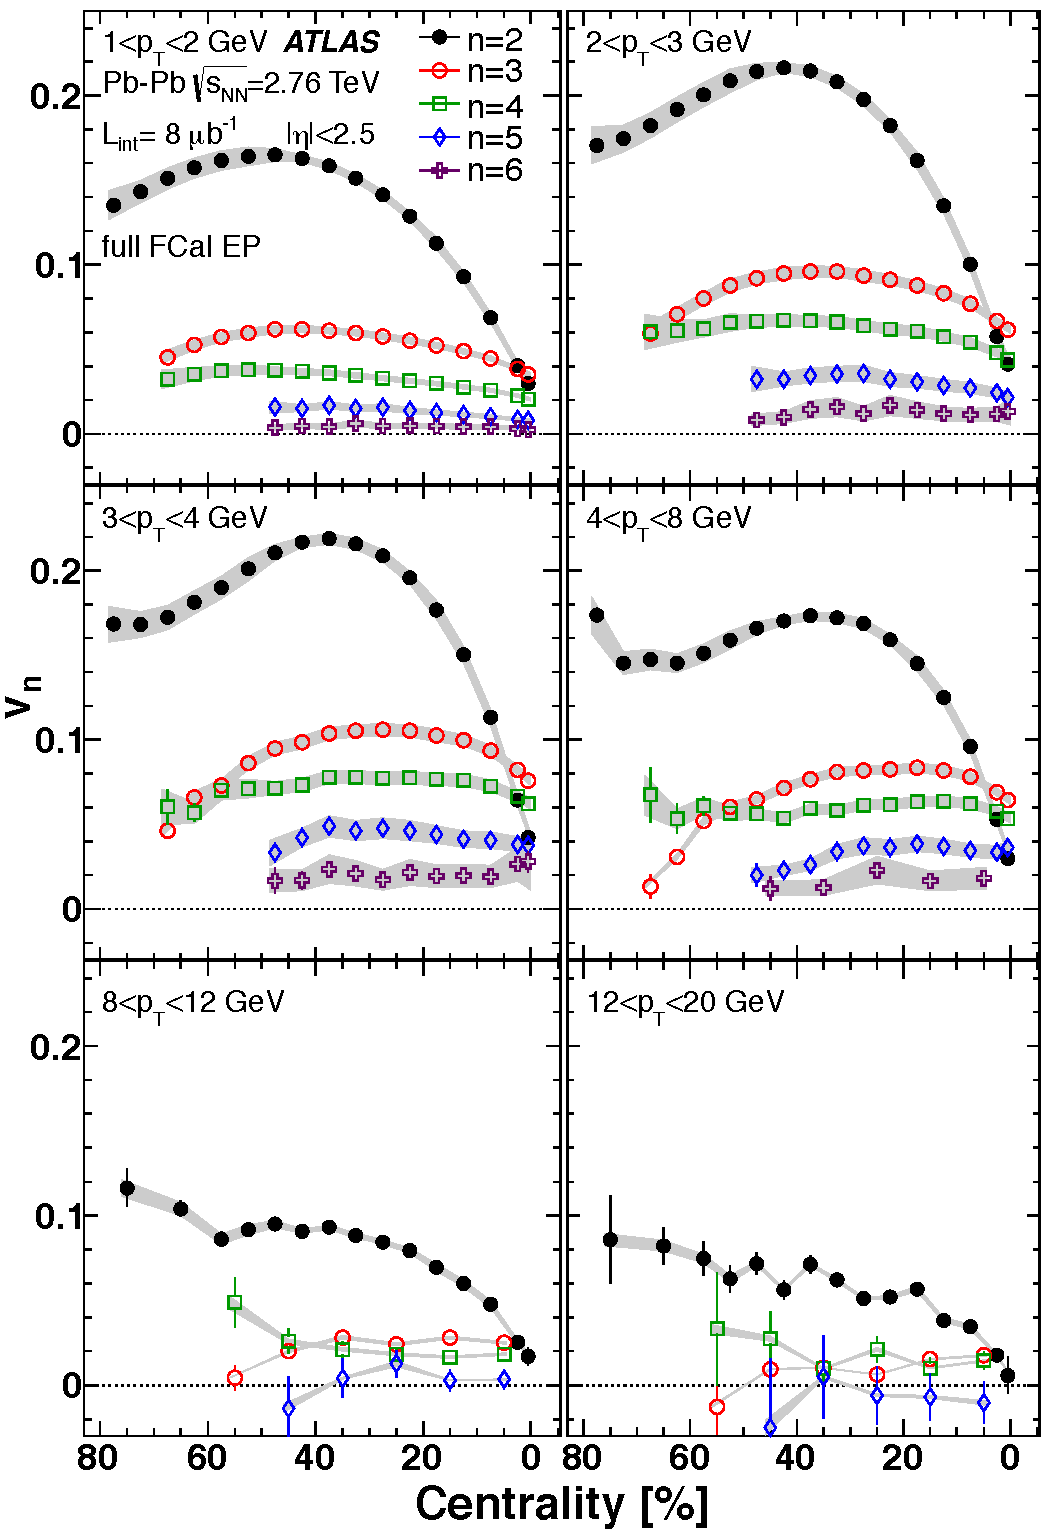
\includegraphics[height=0.6\textwidth]{flowcorrelations_figs/atlas_vn_fig_05.pdf}
\caption[]{(left) ATLAS data showing $v_n(\pT)$ for different centrality intervals and $|\eta|<2.5$, for $n=2-6$.  Very little dependence on $\eta$ is observed~\cite{ATLAS:2012at}.
(right) The same ATLAS data, in \pT\ intervals, showing the approximate centrality dependence of $v_3-v_6$~\cite{ATLAS:2012at}.}
\label{fig:pas:fc:vn}
\end{center}
\end{figure}
Although the realization that $v_2$ was sensitive to fluctuations in the nuclear overlap, particularly from
the event-wise random positions of nucleons in each nuclei, emerged in the mid-2000's, 
several more years elapsed before it was suggested
to look for higher-order harmonic flow, particularly odd-orders~\cite{Alver:2010gr,Qiu:2011iv}.
Many authors argued that symmetric systems
would have a zero $v_1$, $v_3$, $v_5$, etc, but had not yet considered the effect of fluctuations.
By mid-2011, all of the LHC and RHIC experiments had significant measurements of many of the higher-order
contributions, up to $v_6$ which was the limit of the statistics in the 2010 run.

CMS released the first evidence for the presence of higher-order harmonics in the two-particle
correlation function.  ALICE released the first measurements of of $v_3-v_5$ up to $\pT=4$~GeV,
using two and four particle cumulants~\cite{ALICE:2011ab}, and followed up with an extensive study of two-particle
correlations in Ref.~\cite{Aamodt:2011by}.
ATLAS had one of the first large-scale studies of higher harmonics
for unidentified hadrons~\cite{ATLAS:2012at}, measuring up to $v_6$ with both event plane
and two-particle correlations over a wide pseudorapidity and \pT\
range, for the 80\% most central collisions.

The ATLAS data~\cite{ATLAS:2012at} shown in
Figure~\ref{fig:pas:fc:vn}(left) and (right) show the harmonics $v_2 -
v_6$ as a function of \pT\ in centrality intervals from the most
central 0-5\% to the most peripheral 70-80\%.  The the figure on the
left shows that the pattern is consistently the same for all
harmonics: a rapid rise starting at low \pT, a peak around 3~GeV, and
a rapid decrease out to higher $\pT$.  While all of the experiments
have demonstrated that $v_2$ does not necessarily go to zero at high
$\pT$, it remains an open question about the higher harmonics, which
can only be resolved with higher statistics.  The right figure shows
the centrality dependence in small \pT\ intervals, demonstrating that
$v_2$ is fundamentally different than the higher harmonics, having a
much milder centrality dependence.  While $v_2$ mainly reflects the
overall geometric shape of the system, the higher harmonics seem to
mainly reflect fluctuations.  However, the decrease in magnitude with
increasing $n$ is generally thought to reflect the presence of viscous
effects.

\begin{figure}[!tb]
\begin{center}
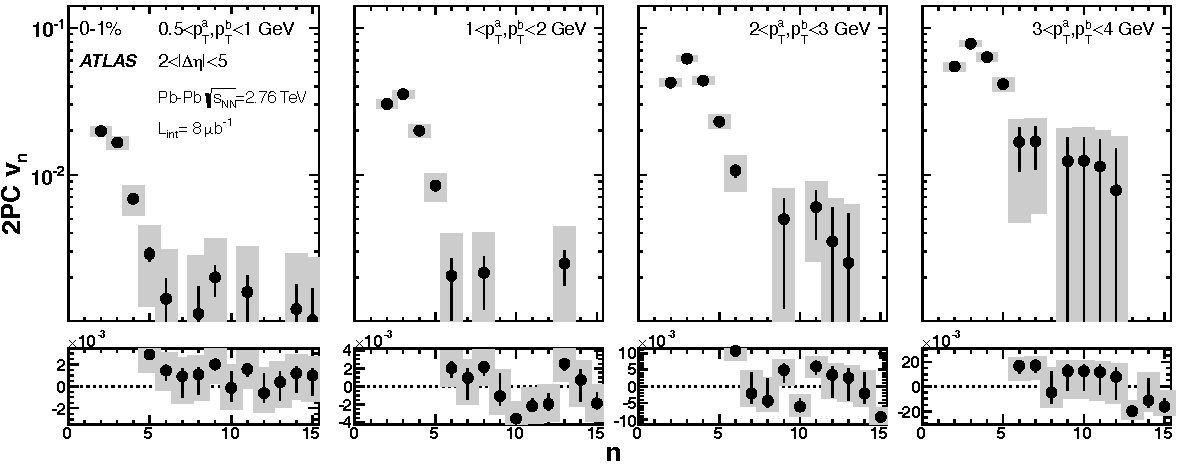
\includegraphics[width=0.98\textwidth]{flowcorrelations_figs/atlas_vn_fig_13.pdf}
\caption[]{
ATLAS data showing the $n$ dependence of $v_n$ in four \pT\ intervals, which are effectively
angular power spectra at different resolution scales.  From Ref.~\cite{ATLAS:2012at}.
}
\label{fig:pas:fc:powerspec}
\end{center}
\end{figure}

\begin{figure}[!tb]
\begin{center}
%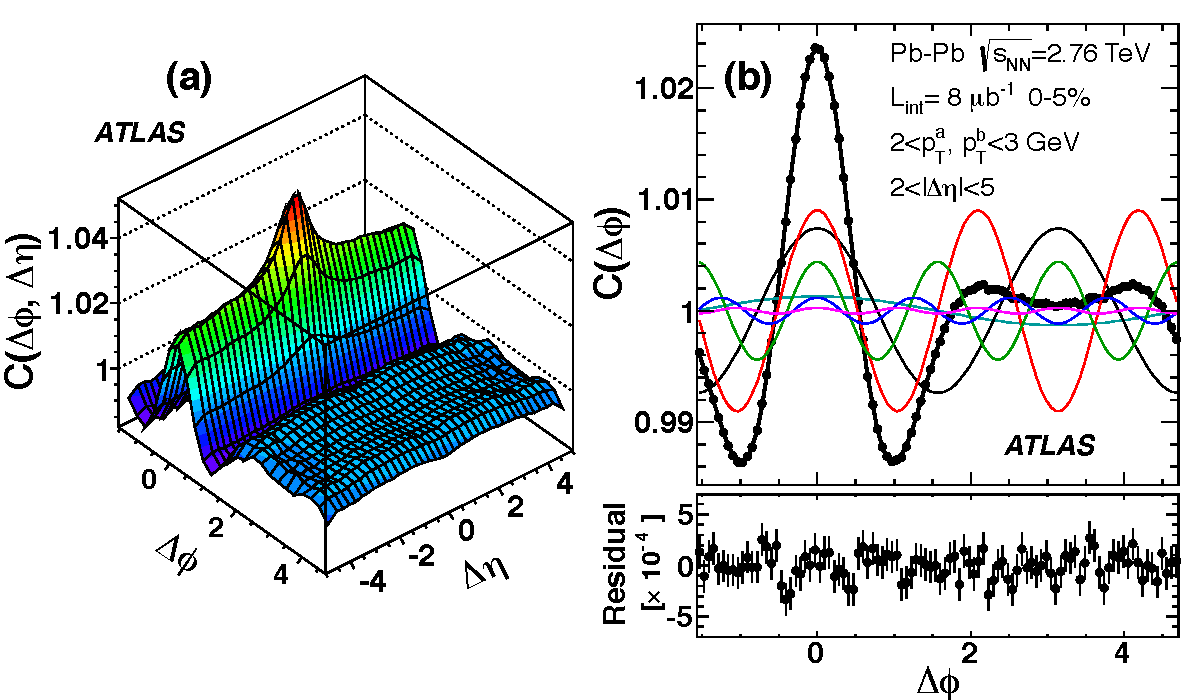
\includegraphics[width=0.58\textwidth]{flowcorrelations_figs/atlas_vn_fig_02a.pdf}
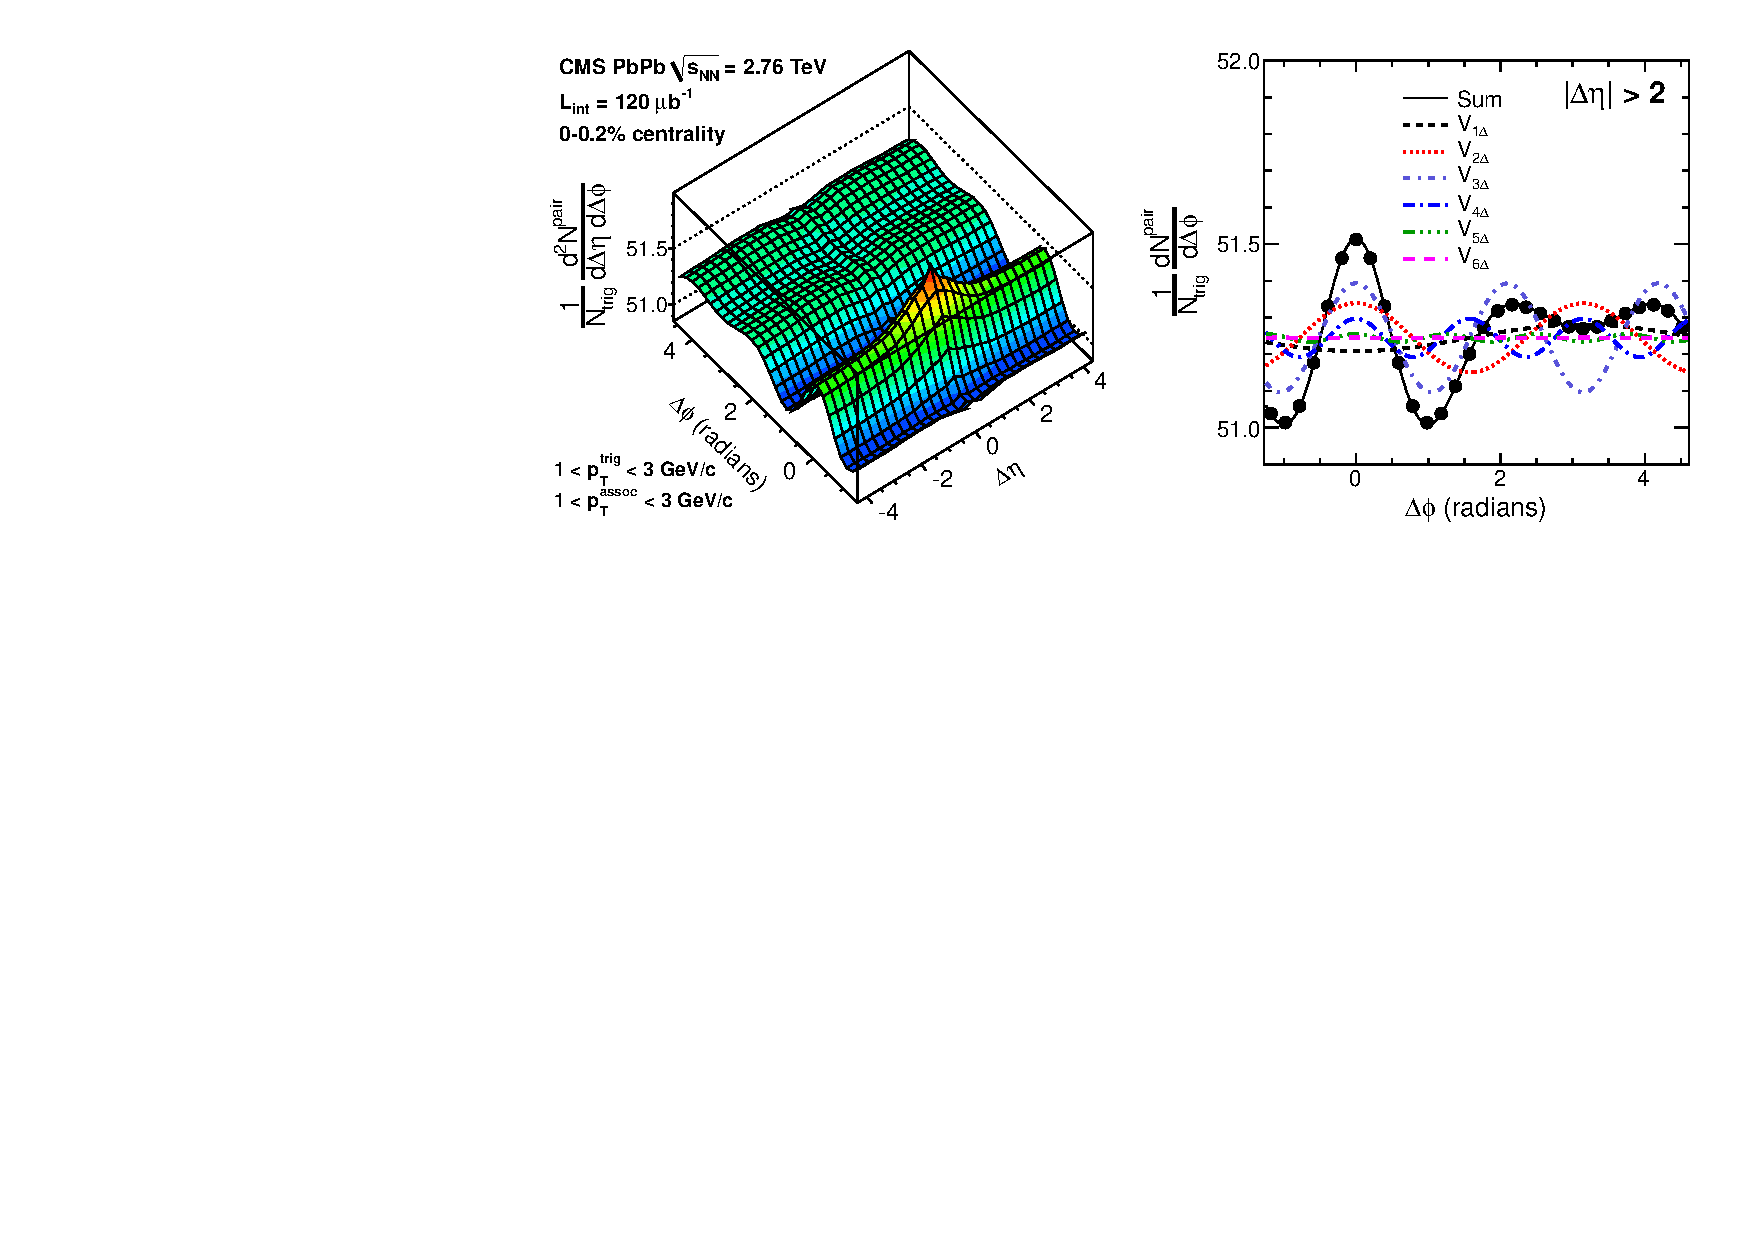
\includegraphics[width=0.68\textwidth]{flowcorrelations_figs/corr1Dfit_UCC_centmin110_centmax1000_20131119.pdf}
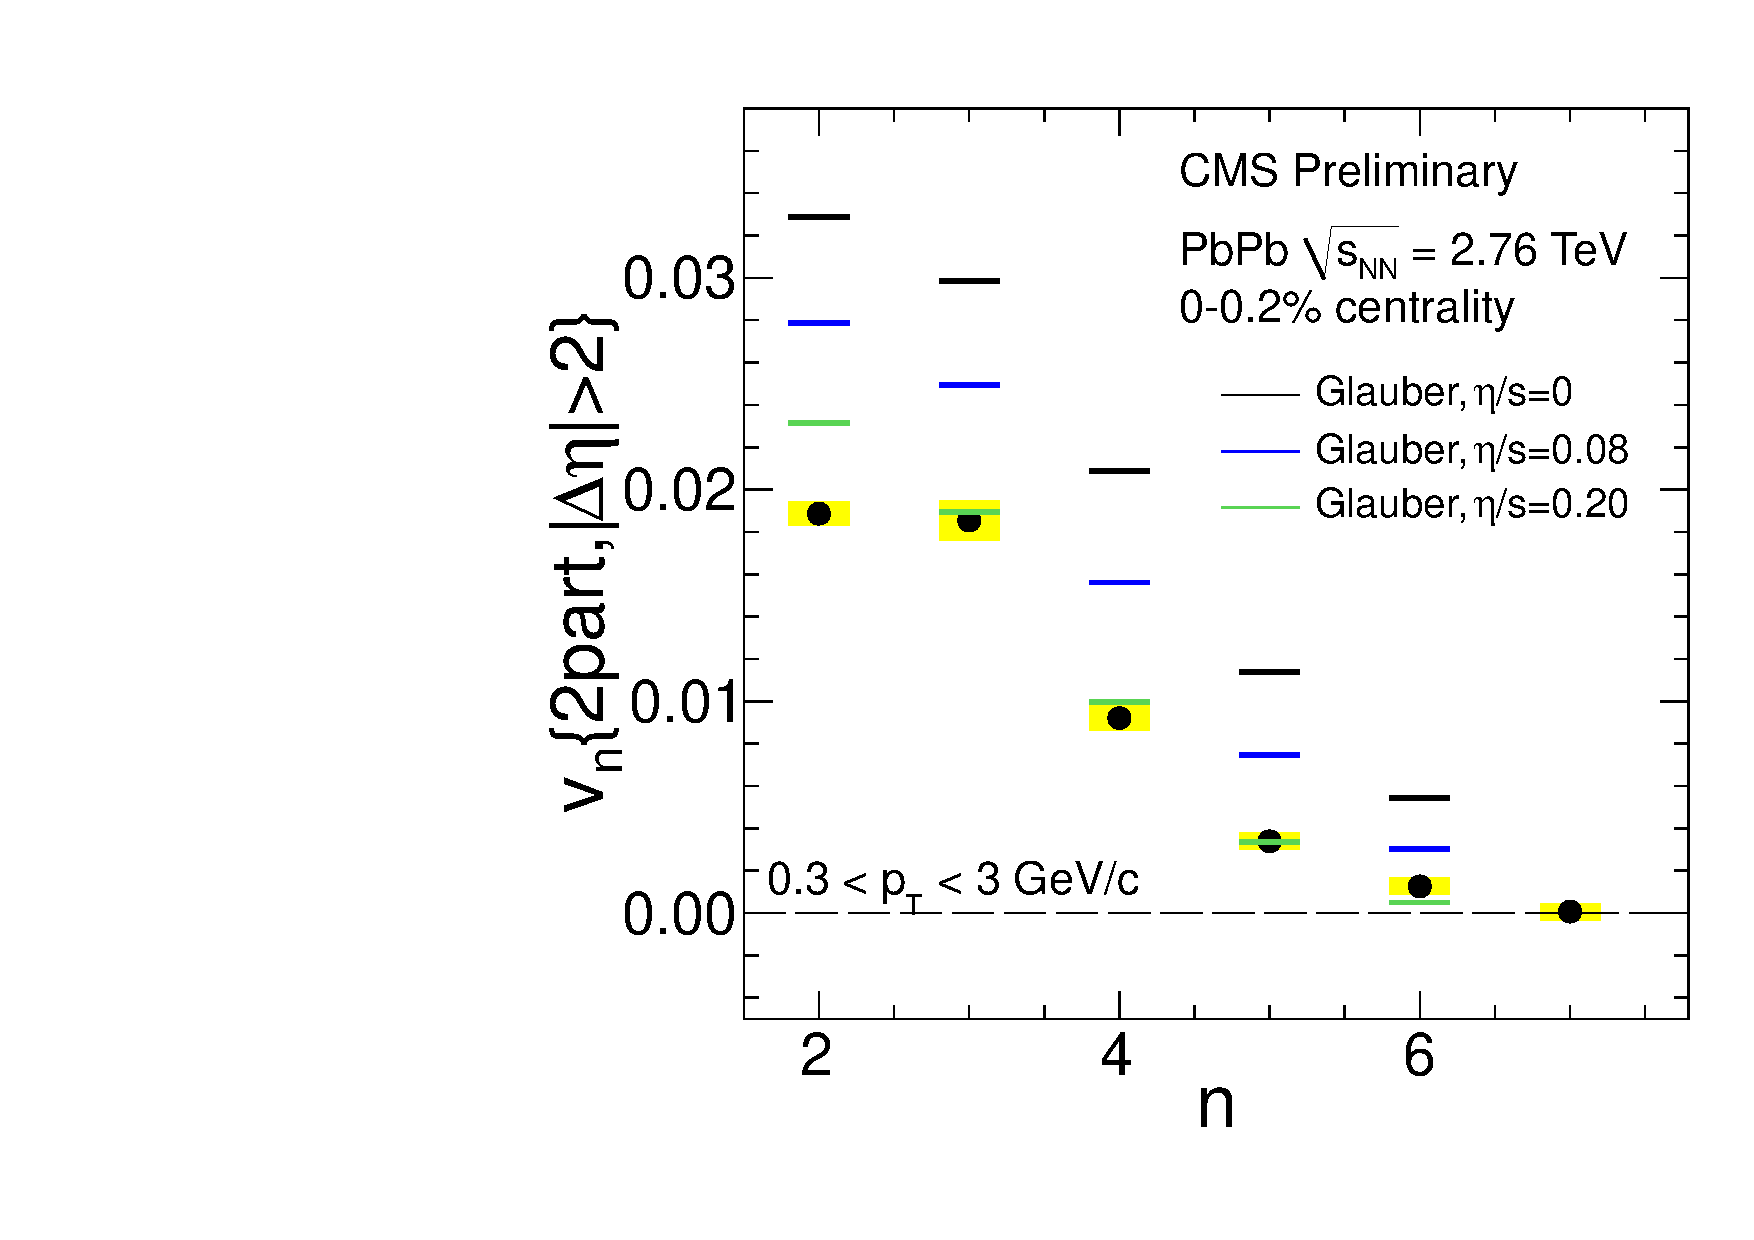
\includegraphics[width=0.3\textwidth]{flowcorrelations_figs/compare_vnn_hydro_luzum_20120810.pdf}
\caption[]{
(left and middle) CMS data showing the decomposition of the 2-particle correlation function,
after requiring the particles have a $\Delta\eta>2$~\cite{CMS:2013bza}.
(right) Results from CMS 2-particle data showing the spectrum of $v_n$ ($n=2-7$) 
for the top 0-0.2\% centrality interval~\cite{CMS:2013bza}.
The data is compared to a hydrodynamical model using Glauber geometry, but
under different assumptions about the viscosity to entropy density ratio.
}
\label{fig:pas:fc:ucc}
\end{center}
\end{figure}

Another representation of this data is given in Figure~\ref{fig:pas:fc:powerspec}, which shows the ``angular power spectrum'',
the $n$ dependence of $v_2(\pT)$ for particular intervals in \pT\ and centrality.  The fall-off with increasing $n$ is a general
feature, of the data which is expected to be driven by viscous corrections that increase with $n$.
CMS has performed a similar study recently with ``ultra central'' collisions, comprising
the top 0.2\% of the minimum bias cross section measured in the high 
luminosity 2011 run~\cite{CMS:2013bza}.  
An example from CMS data showing the 
decomposition of the 2-particle correlation function in the 0-5\% most central
events is shown in Figure~\ref{fig:pas:fc:ucc}(left and middle).
The results shown in Figure~\ref{fig:pas:fc:ucc}(right)
are compared to detailed hydrodynamic calculations under
different assumptions about the initial viscosity to entropy ratio, with
the extreme centrality selection removing most of the effect of the 
the initial shape.

\begin{figure}[!tb]
\begin{center}
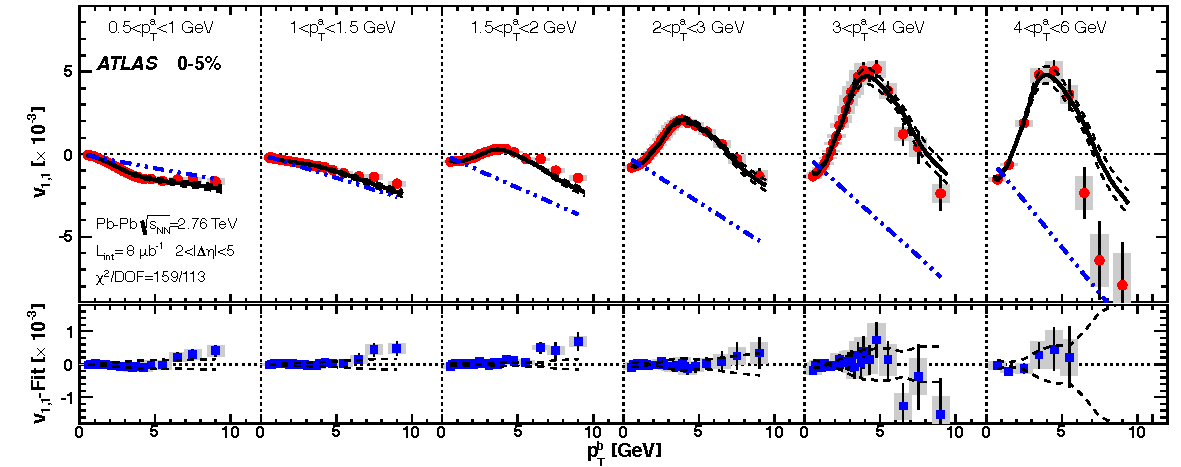
\includegraphics[width=0.98\textwidth]{flowcorrelations_figs/atlas_vn_fig_20a.pdf}
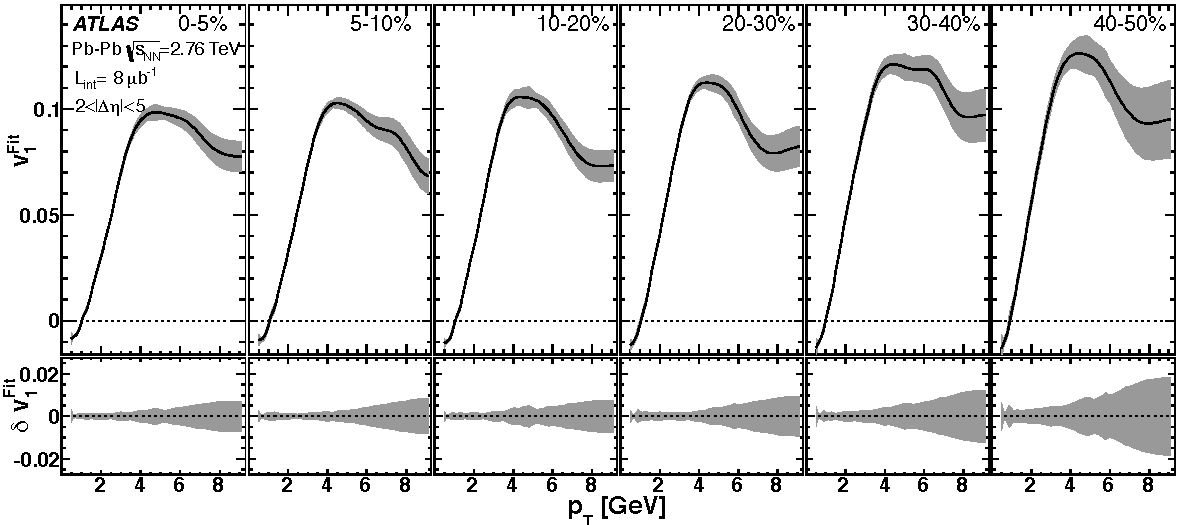
\includegraphics[width=0.93\textwidth]{flowcorrelations_figs/atlas_vn_fig_21.pdf}
\caption[]{ (top) ATLAS data showing the amplitude of $v_{1,1}$ the
  dipole modulation in the 2-particle correlation function, as a
  function of $p^b_T$ for ranges in $p^a_T$.  The fit used to extract
  the functional form of $v_1(\pT)$ is shown~\cite{ATLAS:2012at}.
  (bottom) The extracted functional form of $v_1(\pT)$, from the fits
  shown above, as a function of centrality~\cite{ATLAS:2012at}.  }
\label{fig:pas:fc:v1}
\end{center}
\end{figure}

While the two-particle analyses from ALICE, ATLAS and CMS all utilized a $v_{1,1}$ term in their fits, the first measurements
did not extract a single-particle $v_1$ contribution, since momentum conservation is expected to be a substantial effect.
The first published extraction of $v_1$ from experimental data was performed by a theoretical team using published ALICE data,
doing a fit of the form $V_{1\Delta}(p^a_T,p^b_T) = v_1(p^a_T)v_1(p^b_T) - k p^a_T p^b_T$.
ATLAS also measure directed flow using a similar approach,
fitting $v_1(\pT)$
The value of $v_1$ was also found to vary only modestly with centrality, suggesting it too arises from fluctuations.

\begin{figure}[!tb]
\begin{center}
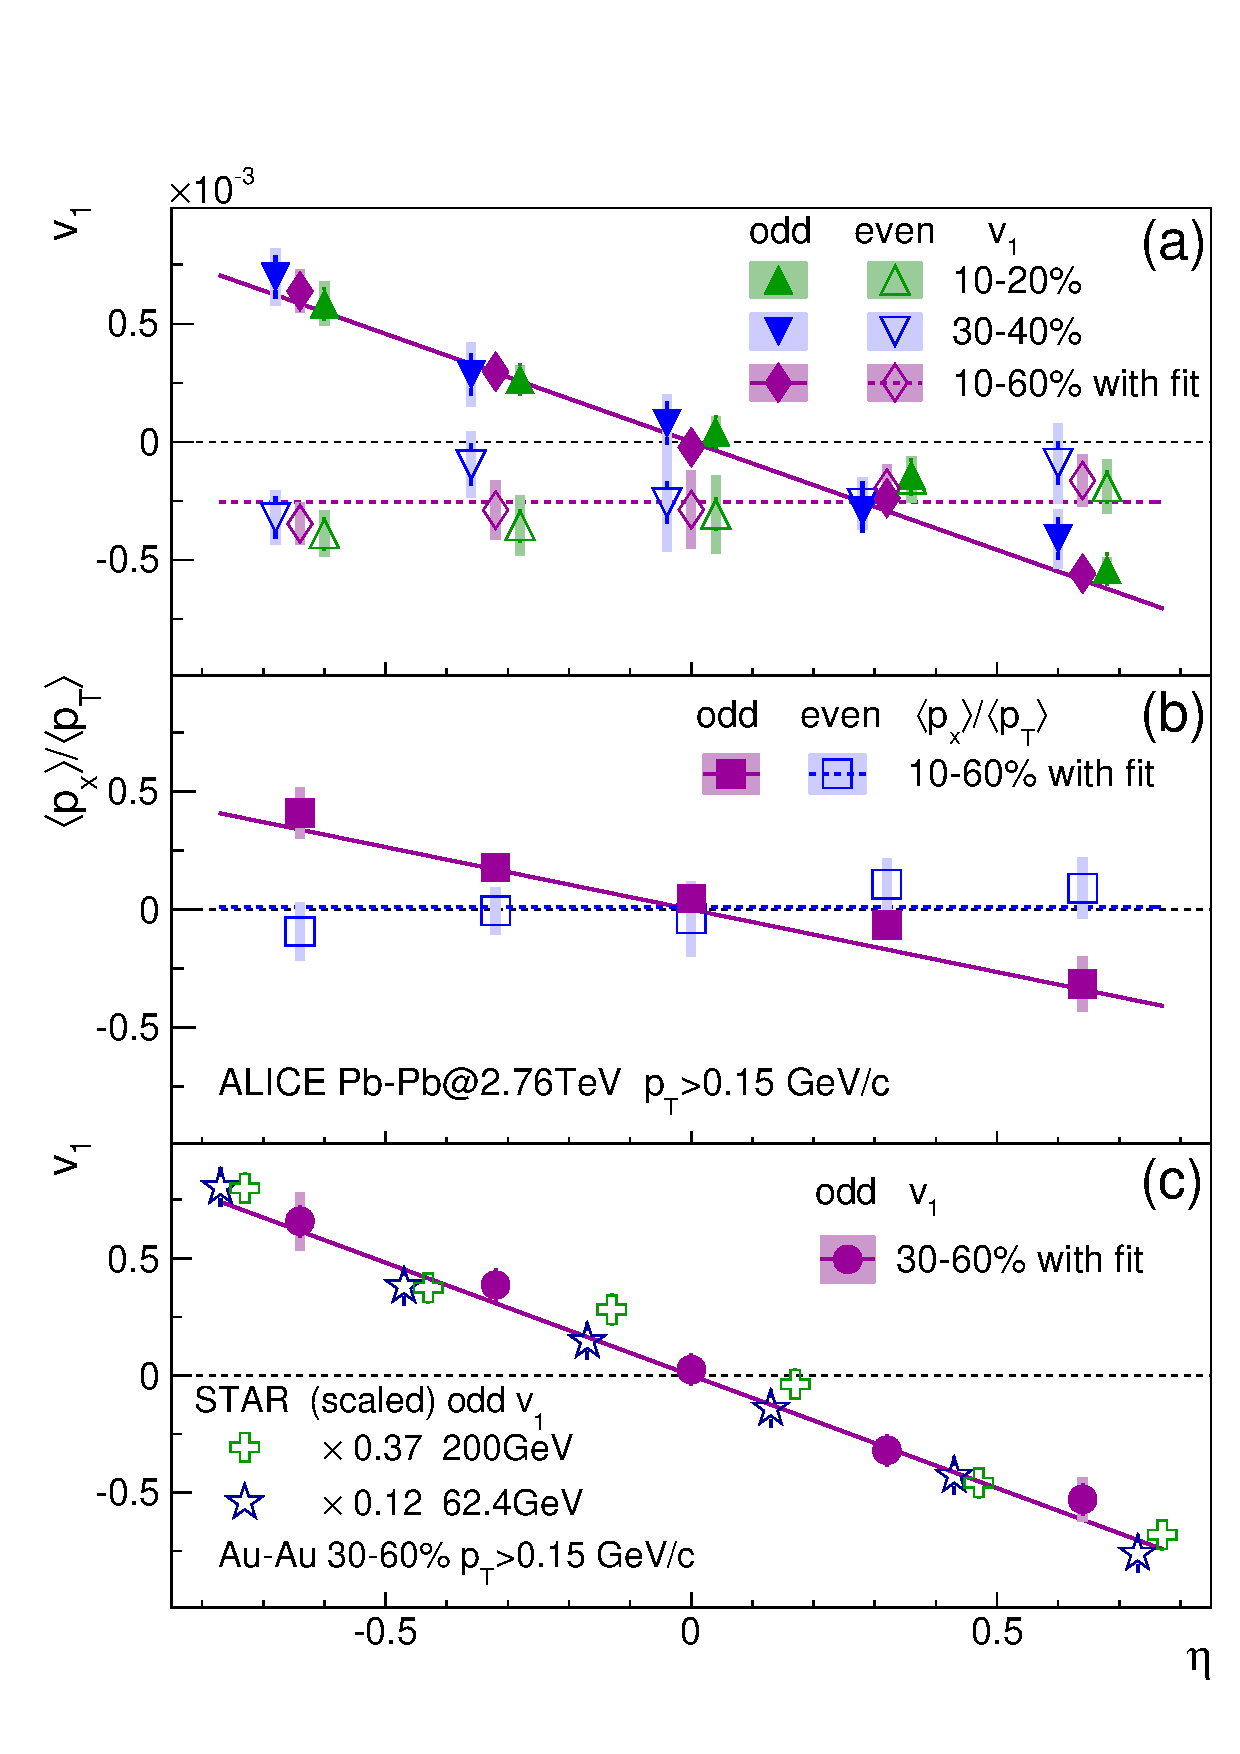
\includegraphics[width=0.4\textwidth]{flowcorrelations_figs/paper_v1_midrapidity_spectators_Figure2.pdf}
\caption[]{ALICE data on directed flow, measured in the plane determined by spectator neutrons
as observed in the ALICE ZDCs.}
\label{fig:pas:fc:v1b}
\end{center}
\end{figure}

The two-particle technique was only able to extract the rapidity-even contribution to $v_1$,
ALICE performed an analysis using the $\Psi_1$ plane determined event-by-event with their
ZDCs, which have a four-fold transverse segmentation~\cite{Abelev:2013cva}.
Figure~\ref{fig:pas:fc:v1b}(a) shows the integrated $v_1$ signal for $\pT>0.15$~GeV as a
function of hadron pseudorapidity, where a linear dependence with a negative slope is observed
for the rapidity-odd $v_1$ signal, and a constant negative value is found for the rapidity-even
$v_1$.  The latter is consistent with the previous extractions of $v_1$ from both the ALICE
and ATLAS data.
As seen in Figure~\ref{fig:pas:fc:v1b}(c) the negative slope is similar to what was found by STAR at
two RHIC energies, but with a much larger slope, suggesting a much smaller ``tilt'' angle
in the x-z plane at higher energies.
Figure~\ref{fig:pas:fc:v1b}(b) shows the mean relative momentum shift in the spectator plane, illustrating
that there is no net momentum flow at $\eta=0$ but it increases with $\eta$ proportionally
to the $v_1$.

\subsection{Flow fluctuations}
\begin{figure}[!tb]
\begin{center}
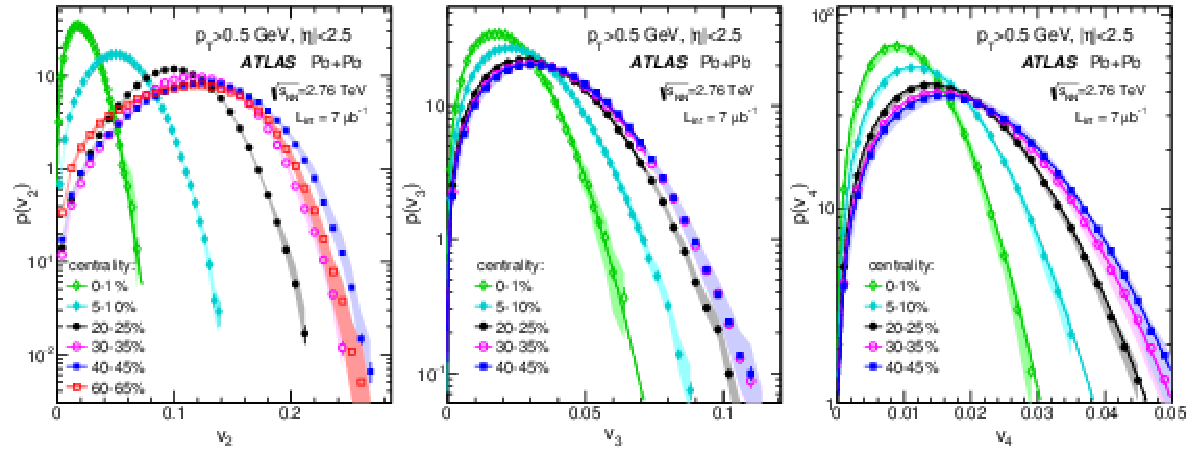
\includegraphics[width=0.98\textwidth]{flowcorrelations_figs/atlas_v2fluc_fig_10.pdf}
\caption[]{
ATLAS data on the event-wise distributions of the harmonic coefficients $v_2 -- v_4$ presented in a selection of
centrality intervals.  From Ref.~\cite{Aad:2013xma}.
}
\label{fig:pas:fc:flowfluc1}
\end{center}
\end{figure}

\begin{figure}[!tb]
\begin{center}
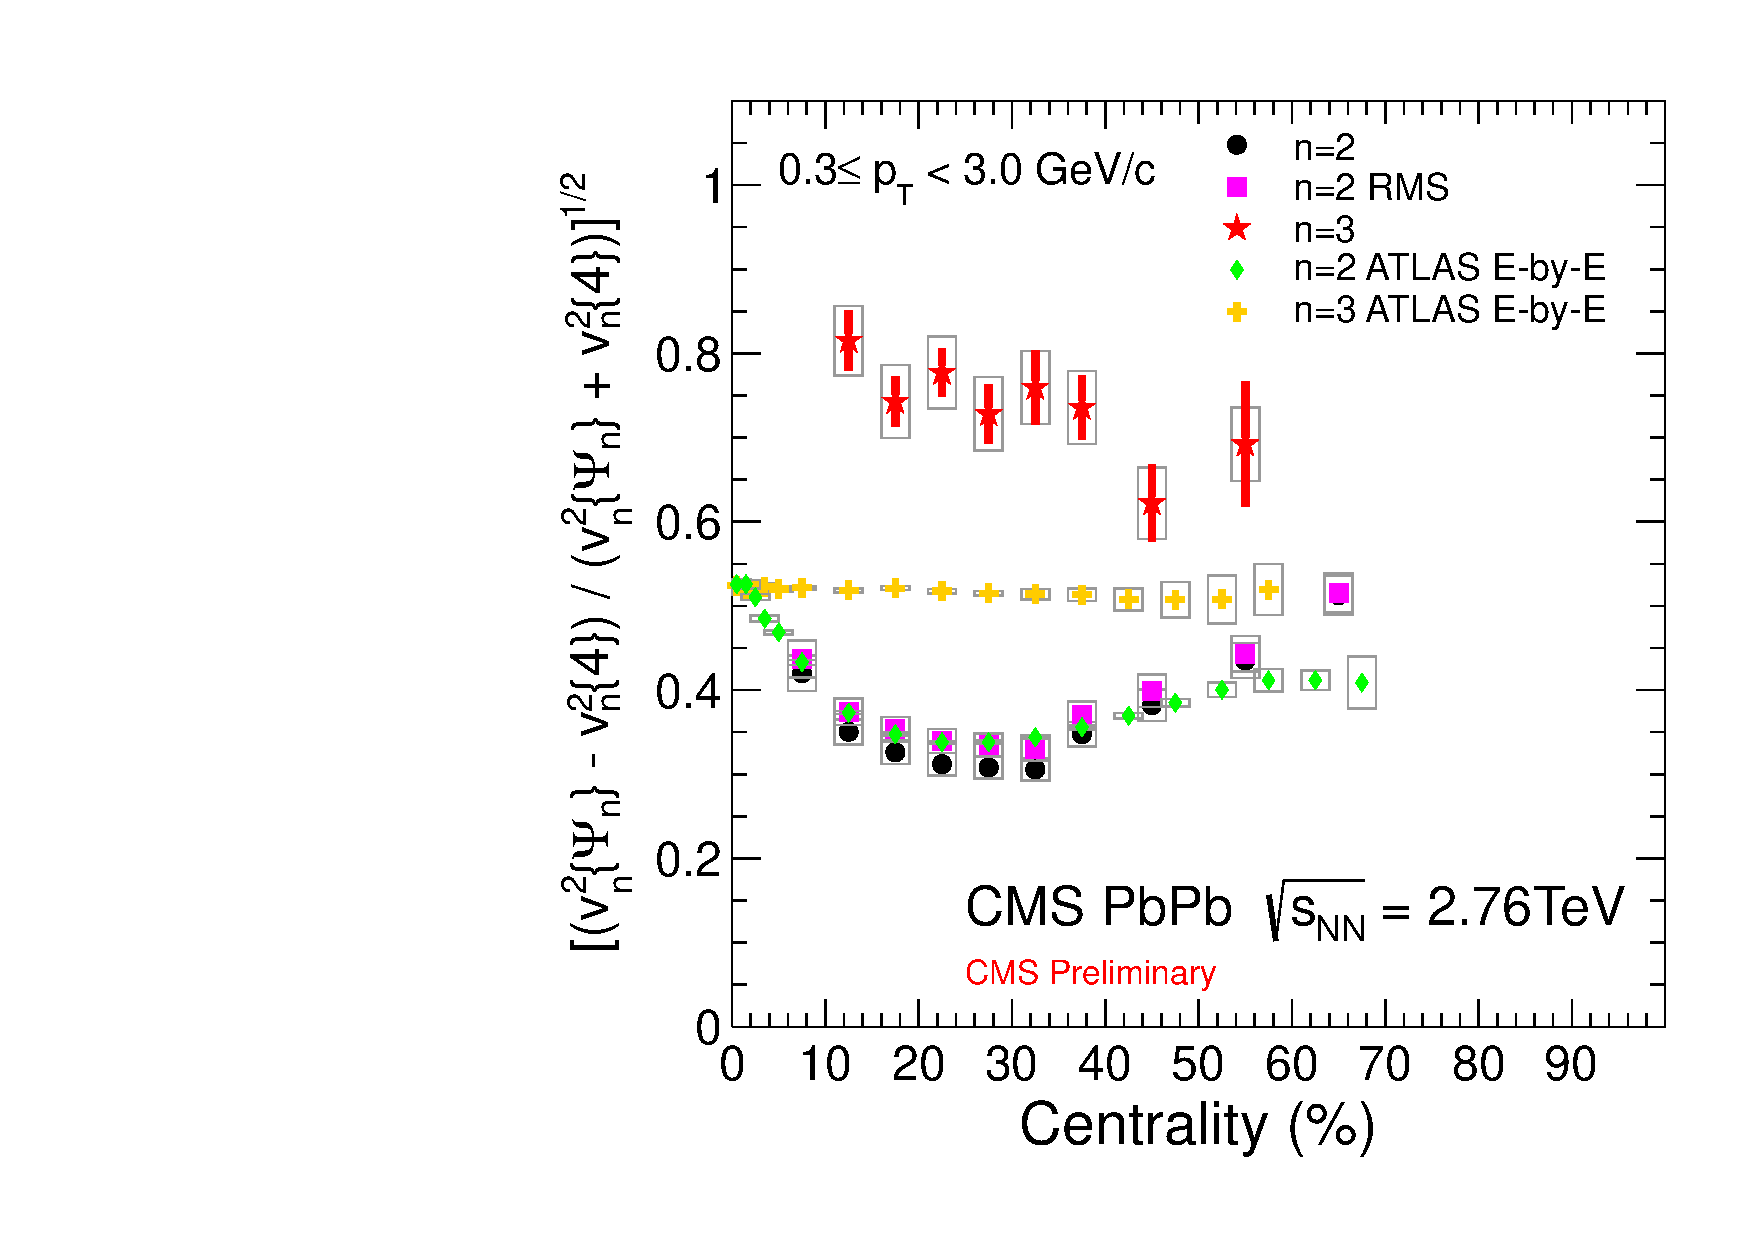
\includegraphics[width=0.40\textwidth]{flowcorrelations_figs/vnSigmaPrelim.pdf}
\raisebox{0.5cm}{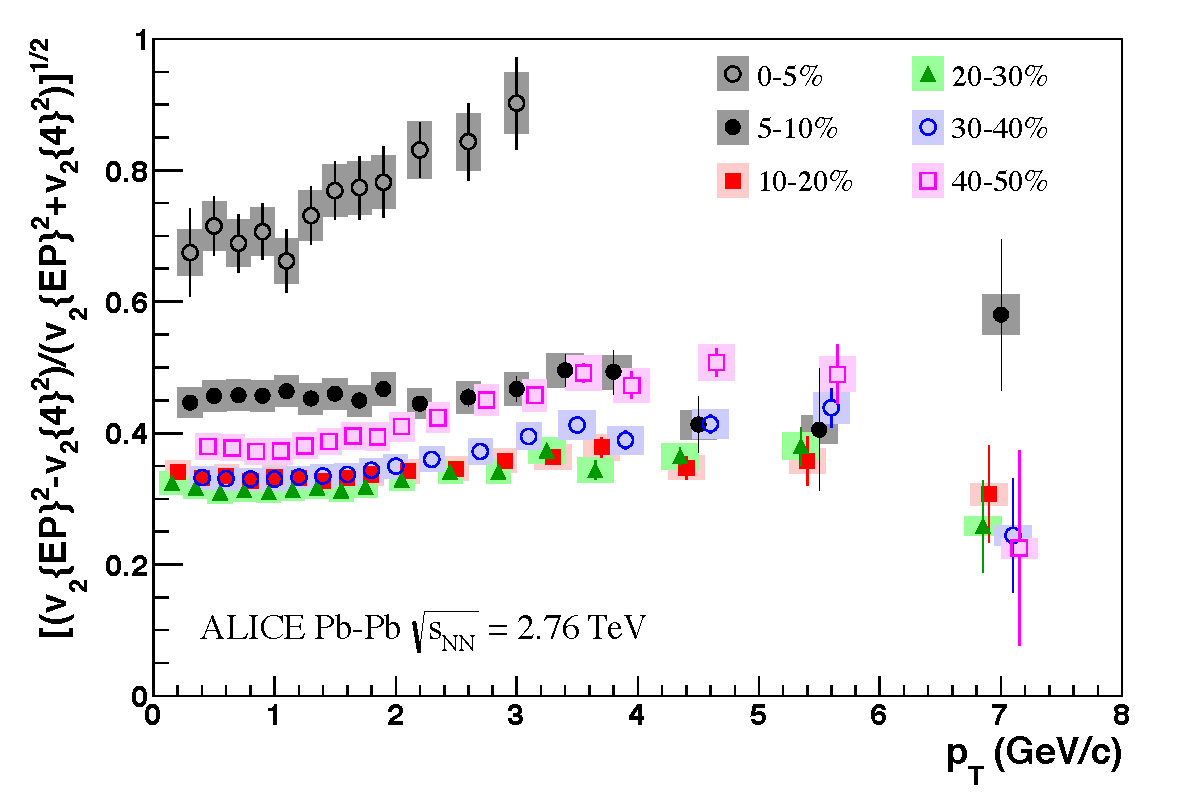
\includegraphics[width=0.55\textwidth]{flowcorrelations_figs/fig3_v2_sigma.pdf}}
\caption[]{
(left) CMS data on the centrality dependence of the standard deviation of $v_2$
divided by the mean, for $0.3 < \pT < 3$~GeV,
extracted via the differences between the EP and cumulant results~\cite{Chatrchyan:2013kba}.
(right) ALICE data on the $\pT$ dependence of the same quantity, out to $\pT=8$~GeV,
for a selected set of centrality
intervals~\cite{Abelev:2012di}.
}
\label{fig:pas:fc:flowfluc2}
\end{center}
\end{figure}

The same geometric fluctuations that lead to the presence of the higher harmonics are also expected to lead to
event-by-event fluctuations in the individual coefficients.  This has been studied using two methods.
ATLAS developed a data-driven method to unfold the measured $v_n$ distributions ($P(v_n)$) with a Bayesian
technique~\cite{Aad:2013xma}.  The distributions $P(v_n)$ are shown in Figure~\ref{fig:pas:fc:flowfluc1} for $v_2$, $v_3$ and $v_4$
for a selected set of centrality intervals.  It is clear that the fluctuations are large in all selected samples.
Although the distributions are not Gaussian, but are rather projections of a 2D Gaussian (also known as a
Bessel-Gaussian distribution),
the distributions are typically quantified using the first two moments, the mean and standard deviation.
These can also be estimated by combining different estimates of $v_n$, in particular using the event-plane
and 4-particle cumulant methods.  Based on the analysis of Ref.{},
the difference between these quantities is twice the variance, while their sum is twice the squared mean.
Figure~\ref{fig:pas:fc:flowfluc2}(left) shows CMS data~\cite{Chatrchyan:2013kba} on $\sigma/\langle v_2 \rangle$ derived
from cumulants, compared with the ATLAS data derived from the fully unfolded distributions.
While the $v_2$ fluctuations compare well between the two methods, the ATLAS and CMS results on $v_3$
are quite different, possibly from the inapplicability of the cumulant approach for this quantity.
The ATLAS results are essentially constant for all centrality intervals at around 0.5, which is the
value one gets ($\sqrt{4/\pi-1}$) if the fluctuations are described by a 2D Gaussian,
projected along the radial direction.
Figure~\ref{fig:pas:fc:flowfluc1}(left) shows ALICE data~\cite{Abelev:2012di} on $\sigma/\langle v_2 \rangle$ derived
using a similar approach as CMS.  For centrality intervals from 5-60\%, the overall magnitude
is similar to that seen by the other experiments.  However, this figure points out that the fluctuations
have essentially no centrality dependence out to moderately large \pT, about 8~GeV, which reaches into
the plateau region typically associated with differential energy loss.




